%\documentclass{acm_proc_article-sp}

%\documentclass{article}

\documentclass{llncs}

\usepackage{wrapfig}
\usepackage{mathpartir}
\usepackage{turnstile}
\usepackage{amssymb}
\usepackage{amsmath}
\usepackage{stmaryrd}
\usepackage{graphicx}
\usepackage{epsfig}
\usepackage{subfigure}
\usepackage{listings}
\usepackage{natbib}
\usepackage{verbatim}
\usepackage[utf8]{inputenc}
\usepackage[T1]{fontenc} 
\usepackage[hyphens]{url}
\lstset{language=ml}
\lstset{commentstyle=\textit}
\lstset{mathescape=true}
\lstset{backgroundcolor=,rulecolor=}
\lstset{frame=single}
\lstset{breaklines=true}
\lstset{basicstyle=\scriptsize\ttfamily}

\DeclareMathOperator{\wf}{wf}
\DeclareMathOperator{\acyclic}{acyclic}
\DeclareMathOperator{\Linear}{Linear}
\DeclareMathOperator{\NonLinear}{NonLinear}
\DeclareMathOperator{\range}{range}
\DeclareMathOperator{\FV}{FV}
\DeclareMathOperator{\LFV}{LFV}
\DeclareMathOperator{\rule-fun}{rule-fun}

\begin{document}

\title{Designing Casanova: a language for games}

\author{
G. Maggiore, \ A. Span\`o, \ R. Orsini, \ G. Costantini, \ M. Bugliesi, \ M. Abbadi \\[1mm]
}

\institute{Universit\`a Ca' Foscari Venezia \\[1mm]
DAIS - Computer Science \\[1mm]
\email{\{maggiore,spano,orsini,costantini,bugliesi,mabbadi\}@dais.unive.it}
}       

\date{}

\maketitle

\begin{abstract}
Games are extremely complex pieces of software which give life to animated virtual worlds. Game developers carefully search the difficult balance between quality and efficiency in their games.

In this paper we present the Casanova language. This language allows the building of games with three important advantages when compared to traditional approaches: simplicity, safety and performance. We will show how to rewrite an official sample of the XNA framework, resulting in a smaller source and higher performance.
\end{abstract}

\begin{comment}
\category{D.1.1}{Programming Techniques}{Applicative (Functional) Programming} 
\category{D.2.2}{Soft\-ware Engineering}{Software Libraries}[Design Tools and Techniques]
\category{D.2.13}{Soft\-ware Engineering}{Reusable Software}[Domain engineering, Reusable libraries, Reuse models]
\category{D.3.3}{Programming Languages}{Language Constructs and Features}
\category{D.3.4}{Pro\-gramming Languages}{Processors}[Optimization, Run-time environments]
\category{H.5.1}{Information Systems}{Information Interfaces and Presentation}[Multimedia Information Systems]

\terms{Games,Performance,Languages}

\keywords{games, optimization}
\end{comment}

\section{Introduction}
\label{sec:introduction}
The number of programming languages available on the market has dramatically increased during the last years. The tiobe index \cite{tiobe2018}, a ranking of programming languages based on their popularity, lists 50 programming languages for 2018. This number is only a small glimpse of the real amount, since it does not take into account several languages dedicated to specific applications. This growth has brought a further need for new compilers that are able to translate programs written in those languages into executable code. The goal of this work is to investigate how the development speed of a compiler can be boosted by employing meta-compilers, programs that generalize the task performed by a normal compiler. In particular the goal of this research is creating a meta-compiler that significantly reduces the amount of code needed to define a language and its compilation steps, while maintaining acceptable performance.

This chapter introduces the issue of expressing the solution of problems in terms of algorithms in Section \ref{sec:ch1_algorithms}. Then we proceed by defining how the semi-formal definition of an algorithm must be translated into code executable by a processor (Section \ref{sec:ch1_programming_languages}). In this section we discuss the advantages and disadvantages of using different kinds of programming languages with respect to their affinity with the specific hardware architecture and the scope of the domain they target. In Section \ref{sec:ch1_compilers} we explain the reason behind compilers and we explain why building a compiler is a time-consuming task. In Section \ref{sec:ch1_metacompilers} we introduce the idea of meta-compilers as a further step into generalizing the task of compilers. In this section we also explain the requirements, benefits, and the relevance as a scientific topic. Finally in Section \ref{sec:ch1_problem_statement} we formulate the problem statement and the research questions that this work will answer.

\section{Algorithms and problems}
\label{sec:ch1_algorithms}
Since the ancient age, there has always been the need of describing the sequence of activities needed to perform a specific task \cite{barbin2012history}, to which we refer with the name of \textit{Algorithm}. The allegedly most ancient known example of this dates back to the Ancient Greek, when Hero invented an algorithm to perform the factorization and the approximation of the square root, discovered also by other civilizations \cite{ bailey2012ancient, smith1923history} . Regardless of the specific details of each algorithm, one needs to use some kind of language  to define the sequence of steps to perform. In the past people used natural language to describe such steps but, with the advent of the computer era, the choice of the language has been strictly connected with the possibility of its implementation. Natural languages are not suitable for the implementation, as they are known to be verbose and ambiguous \cite{church1982coping, resnik1999semantic}. For this reason, several kind of formal solutions have been employed, which are described below.

\subsubsection*{Flow charts}
A flow chart is a diagram where the steps of an algorithm are defined by using boxes of different kinds, connected by arrows to define their ordering in the sequence. The boxes are rectangular-shaped if they define an \textit{activity} (or processing step), while they are diamond-shaped if they define a \textit{decision}. A rectangle with rounded corners denotes the initial step. An example of a flow chart describing how to sum the numbers in a sequence is described in Figure \ref{fig:ch1_flow_chart}.

\begin{figure}
	\centering
	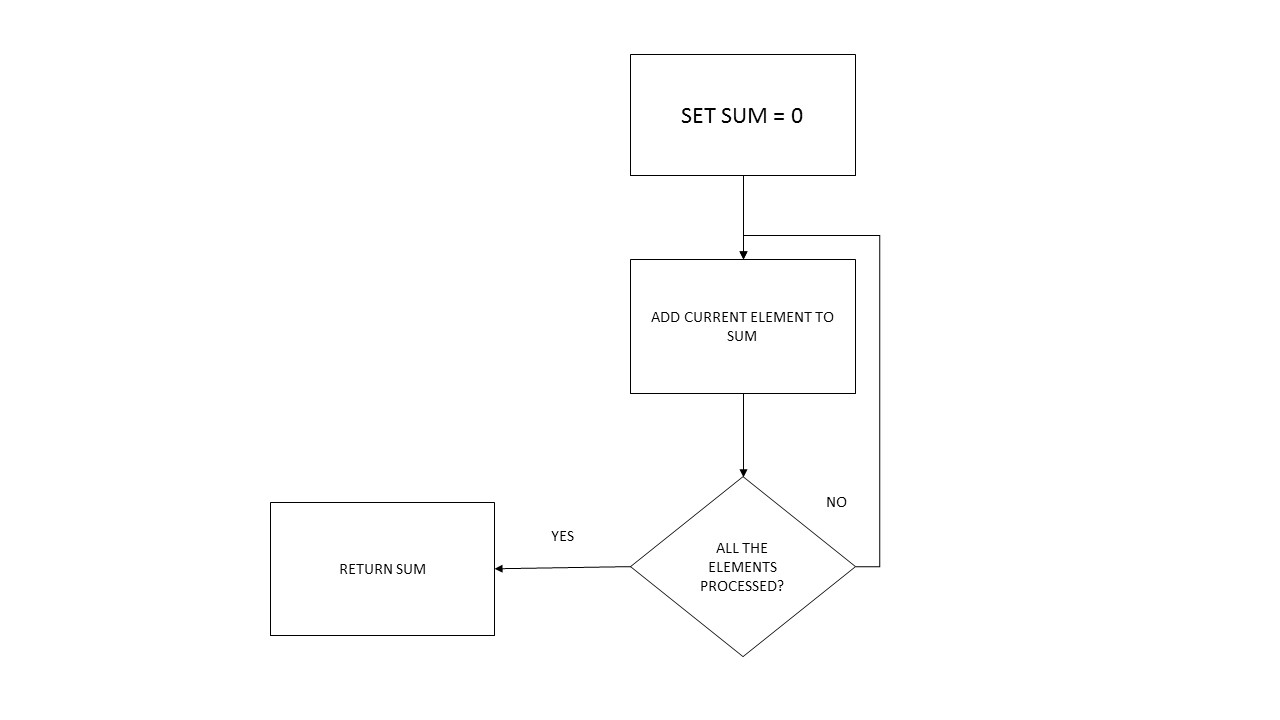
\includegraphics[width = \textwidth]{Figures/flow_chart}
	\caption{Flow chart for the sum of a sequence of numbers}
	\label{fig:ch1_flow_chart}
\end{figure}

\subsubsection*{Pseudocode}
Pseudocode is a semi-formal language that might contain also statements expressed in natural language and omits system specific code like opening file writers, printing messages on the standard output, or even some data structure declaration and initialization. It is intended mainly for human reading rather than machine reading. The pseudocode to sum a sequence of numbers is shown in Algorithm \ref{alg:ch1_pseudocode}.

\begin{algorithm}
	\caption{Pseudocode to perform the sum of a sequence of integer numbers}
	\label{alg:ch1_pseudocode}
	\begin{algorithmic}
		\Function{SumIntegers}{$l \text{ list of integers}$}
			\State $sum \gets 0$
			\ForAll {$x \text{ in } l$}
				\State $sum \gets sum + x$
			\EndFor
			\State \Return $sum$
		\EndFunction
	\end{algorithmic}
\end{algorithm}

\subsubsection*{Advantages and disadvantages}
Using flow charts or pseudo-code has the advantage of being able to define an algorithm in a way which is very close to the abstractions employed when using natural language: a flow chart combines both the use of natural language and a visual interface to describe an algorithm, pseudo-code allows to employ several abstractions and even define some steps in terms of natural language. The drawback of these two formal representations is that, when it comes to the implementation, the definition of the algorithm must be translated by hand into code that the hardware is able to execute. This could be done by implementing the algorithm in a low-level or high-level programming language. This process affects at different levels how the logic of the algorithm is presented, as explained further.

\section{Programming languages}
\label{sec:ch1_programming_languages}
A programming language is a formal language that is used to define instructions that a machine, usually a computer, must perform in order to produce a result through computation \cite{mordechai1996, narasimhan1967programming, oxford2008}. There is a wide taxonomy used to classify programming languages depending on their use \cite{kelleher2005lowering, myers1986visual, myers1990taxonomies}, but all can be grouped according to two main characteristics: the level of abstraction, or how close to the specific targeted hardware they are, and the domain, which defines the range of applicability of a programming language. In the following sections we give an exhaustive explanation of the aforementioned characteristics.

\subsection{Low-level programming languages}
\label{subsec:ch1_ll_languages}
A low-level programming language is a programming language that provides little to no abstraction from the hardware architecture of a processor. This means that it is strongly connected with the instruction set of the targeted machine, the set of instructions a processor is able to execute. These languages are divided into two sub-categories: \textit{first-generation} and \textit{second-generation} languages:

\subsubsection*{First-generation languages}
\textit{Machine code} falls into the category of first-generation languages. In this category we find all those languages that do not require code transformations to be executed by the processor. These languages were used mainly during the dawn of computer age and are rarely employed by programmers nowadays. Machine code is made of stream of binary data, that represents the instruction codes and their arguments \cite{guide2011intel, seal2001arm}. Usually this stream of data is treated by programmers in hexadecimal format, which is then remapped into binary code. The programs written in machine code were once loaded into the processor through a front panel, a controller that allowed the display and alteration of the registers and memory (see Figure \ref{fig:ch1_front_panel}). An example of machine code for a program that computes the sum of a sequence of integer numbers can be seen in Listing \ref{lst:ch1_machine_code}.

\begin{figure}
	\centering
	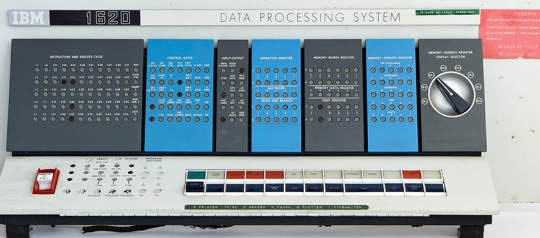
\includegraphics[width = \textwidth]{Figures/ch1_front_panel}
	\caption{Front panel of IBM 1620}
	\label{fig:ch1_front_panel}
\end{figure}

\begin{minipage}{\linewidth}
\begin{lstlisting}[numbers = left, caption = Machine code to compute the sum of a sequence of numbers, label = lst:ch1_machine_code]
 00075	c7 45 b8 00 00
 00 00
 0007c	eb 09	
 0007e	8b 45 b8
 00081	83 c0 01
 00084	89 45 b8
 00087	83 7d b8 0a
 0008b	7d 0f
 0008d	8b 45 b8
 00090	8b 4d c4
 00093	03 4c 85 d0
 00097	89 4d c4
 0009a	eb e2
\end{lstlisting}
\end{minipage}

\subsubsection*{Second-generation languages}
The languages in this category provides an abstraction layer over the machine code by expressing processor instructions with mnemonic names both for the instruction code and the arguments. For example, the arithmetic sum instruction \texttt{add} is the mnemonic name for the instruction code \texttt{0x00} in \texttt{x86} processors. Among these languages we find \textit{Assembly}, that is mapped with an \textit{Assembler} to machine code. The Assembler can load directly the code or link different \textit{object files} to generate a single executable by using a \textit{linker}. An example of assembly \texttt{x86} code corresponding to the machine code in Listing \ref{lst:ch1_machine_code} can be found in Listing \ref{lst:ch1_assembly_code}. You can see that the code in the machine code \texttt{00081	83 c0 01} at line 5 has been replaced by its mnemonic representation in Assembly as \texttt{add	eax, 1}.

\begin{minipage}{\linewidth}
\begin{lstlisting}[numbers = left, caption = Assembly x86 code to compute the sum of a sequence of numbers, label = lst:ch1_assembly_code]
mov	DWORD PTR _i$1[ebp], 0
jmp	SHORT $LN4@main
$LN2@main:
mov	eax, DWORD PTR _i$1[ebp]
add	eax, 1
mov	DWORD PTR _i$1[ebp], eax
$LN4@main:
cmp	DWORD PTR _i$1[ebp], 10			; 0000000aH
jge	SHORT $LN3@main
mov	eax, DWORD PTR _i$1[ebp]
mov	ecx, DWORD PTR _sum$[ebp]
add	ecx, DWORD PTR _numbers$[ebp+eax*4]
mov	DWORD PTR _sum$[ebp], ecx
jmp	SHORT $LN2@main
\end{lstlisting}
\end{minipage}

\subsubsection*{Advantages and disadvantages}
Writing a program in low-level programming languages might produce programs that are generally more efficient than their high-level counterparts, as ad-hoc optimizations are possible. However, the high-performance comes at great costs: (\textit{i}) the programmer must be an expert of the underlying architecture and of the specific instruction set of the processor, (\textit{ii}) the program loses portability because the low-level code is tightly bound to the specific hardware architecture it targets, (\textit{iii}) the logic and readability of the program is hidden among the details of the instruction set itself, and (\textit{iv}) developing a program in assembly requires a considerable effort in terms of time and debugging \cite{frampton2009demystifying}: assembly lacks any abstraction from the concrete hardware architecture, such as a type system, that partially ensures the correctness of the program or high-level constructs that allow to manipulate the execution of the program.

\subsection{High-level programming languages}
\label{subsec:ch1_hl_languages}
A high-level programming language is a programming language that offers a high level of abstraction from the specific hardware architecture of the machine. Unlike machine code (and in some way also assembly), high-level languages are not directly executable by the processor and they require some kind of translation process into machine code. The level of abstraction offered by the language defines how high level the language is. Several categories of high-level programming language exist, but the main one are described below.

\subsubsection*{Imperative programming languages}
\textit{Imperative programming languages} model the computation as a sequence of statements that alter the state of the program (usually the memory state). A program in such languages consists then of a sequence of \textit{commands}. Notable examples are FORTRAN, C, and PASCAL. An example of the program used in Listing \ref{lst:ch1_machine_code} and \ref{lst:ch1_assembly_code} written in C can be seen in Listing \ref{lst:ch1_c_code}. Line 5 to 9 corresponds to the Assembly code in Listing \ref{lst:ch1_assembly_code}.

\begin{lstlisting}[numbers = left, caption = C code to compute the sum of a sequence of numbers, label = lst:ch1_c_code]
int main()
{
  int numbers[10] = { 1, 6, 8, -2, 4, 3, 0, 1, 10, -5 };
  int sum = 0;
  for (int i = 0; i < 10; i++)
  {
    sum += numbers[i];
  }
  printf("%d\n", sum);
}
\end{lstlisting}

\subsection*{Declarative programming languages}
\textit{Declarative programming languages} are antithetical to those based on imperative programming, as they model computation as an evaluation of expressions and not as a sequence of commands to execute. Declarative programming languages are called as such when they are side-effects free or referentially transparent. The definition of referential transparency varies \cite{quine2013word}, but it is usually explained with the substitution principle, which states that a language is referentially transparent if any expression can be replaced by its value without altering the behaviour of the program \cite{mitchell2003concepts}. For instance, the following sentences in natural language are both true

\begin{lstlisting}
Cicero = Tullius

''Cicero`` contains six letters
\end{lstlisting} 

\noindent
but they are not referentially transparent, since replacing the last name with the middle name falsifies the second sentence.

A similar situation in programming languages is met when considering variable assignments: the statement

\begin{lstlisting}
x = x + 5
\end{lstlisting}

\noindent
is not referentially transparent. Let us assume this statement appears twice in a program and that at the beginning x = 0. Clearly the expression \texttt{x + 5} results in the value 5 the first time, but the second time the same statement is executed the expression has value 10. Thus replacing all the occurrences of \texttt{x + 5} with 5 is wrong, which is why imperative languages are not referentially transparent. A more rigorous definition of referential transparency can be found in \cite{sondergaard1990referential}.

Declarative programming languages are often compared to imperative programming languages by stating that declarative programming defines \textit{what} to compute and not \textit{how} to compute it. This family of languages include \textit{functional programming}, \textit{logic programming}, and \textit{database query languages}. Notable examples are F\#, Haskell, Prolog, SQL, and Linq (which is a query language embedded in C\#). Listing \ref{lst:ch1_fsharp_code_rec} shows the code to perform the sum of a sequence of integer numbers in F\# with a recursive function. Higher-order functions, such as \texttt{fold}, allow even to capture the same recursive pattern into a single function as shown in Listing \ref{lst:ch1_fsharp_code_fold}. Both implementations are referentially transparent.

\begin{lstlisting}[caption = Recursive F\# code to compute the sum of a sequence of numbers, label = lst:ch1_fsharp_code_rec]
let rec sumList l =
  match l with
  | [] -> 0
  | x :: xs -> x + (sumList xs)
\end{lstlisting}

\begin{lstlisting}[caption = F\# code to compute the sum of a sequence of numbers using higher-order functions, label = lst:ch1_fsharp_code_fold]
let sumList l = l |> List.fold (+) 0
\end{lstlisting}

\subsection{General-purpose vs Domain-specific languages}
\label{sec:ch1_dsl}
\textit{General-purpose languages} are defined as languages that can be used across different application domains and lack abstractions that specifically target elements of a single domain. Example of these are languages such as C, C++, C\#, and Java. Although several applications are still being developed by using general-purpose programming languages, in several contexts it is more convenient to rely on \textit{domain-specific languages}, because they offer abstractions relative to the problem domain that are unavailable in general-purpose languages \cite{van2000domain, voelter2013dsl}. Notable examples of the use of domain-specific languages are listed below.

\subsubsection*{Graphics programming}
Rendering a scene in a 3D space is often performed by relying on dedicated hardware. Modern graphics processors rely on shaders to create various effects that are rendered in the 3D scene. Shaders are written in domain-specific languages, such as GLSL or HLSL \cite{glhl2014, hlsl2018, hlslref2018}, that offer abstractions to compute operations at GPU level that are often used in computer graphics, such as vertices and pixel transformations, matrix multiplications, and interpolation of textures. Listing \ref{lst:ch1_hlsl_code} shows the code to implement light reflections in HLSL. At line 4 you can, for example, see the use of matrix multiplication provided as a language abstraction in HLSL.

\begin{lstlisting}[numbers = left, caption = HLSL code to compute the light reflection, label = lst:ch1_hlsl_code]
VertexShaderOutput VertexShaderSpecularFunction(VertexShaderInput input, float3 Normal : NORMAL)
{
  VertexShaderOutput output;
  float4 worldPosition = mul(input.Position, World);
  float4 viewPosition = mul(worldPosition, View);
  output.Position = mul(viewPosition, Projection);
  float3 normal = normalize(mul(Normal, World));
  output.Normal = normal;
  output.View = normalize(float4(EyePosition,1.0f) - worldPosition);
  return output;
}
\end{lstlisting}

\subsubsection*{Game programming}
Computer games are a field where domain-specific languages are widely employed, as they contain complex behaviours that often require special constructs to model timing event-based primitives, or to execute tasks in parallel. These behaviours cannot be modelled, for performance reasons, by using threads. Therefore, in the past, domain-specific languages which provide these abstractions have been implemented \cite{nwnlexicon2018, jass2011, unrealscript2018, sqf2018}. In Listing \ref{lst:ch1_sqf_code} an example of the SQF domain-specific language for the game ArmA2 is shown. This language offers abstractions to wait for a specific amount of time, to wait for a condition, and to spawn scripts that run in parallel to the callee, that you can respectively see at lines 18, 12, and 10.

\begin{lstlisting}[numbers = left, caption = ArmA 2 scripting language, label = lst:ch1_sqf_code]
"colorCorrections" ppEffectAdjust [1, pi, 0, [0.0, 0.0, 0.0, 0.0], [0.05, 0.18, 0.45, 0.5], [0.5, 0.5, 0.5, 0.0]];  
"colorCorrections" ppEffectCommit 0;  
"colorCorrections" ppEffectEnable true;

thanatos switchMove "AmovPpneMstpSrasWrflDnon";
[[],(position tower) nearestObject 6540,[["USMC_Soldier",west]],4,true,[]] execVM "patrolBuilding.sqf";
playMusic "Intro";

titleCut ["", "BLACK FADED", 999];
[] Spawn 
{
	waitUntil{!(isNil "BIS_fnc_init")};
	[
	  localize "STR_TITLE_LOCATION" ,
	  localize "STR_TITLE_PERSON",
	  str(date select 1) + "." + str(date select 2) + "." + str(date select 0)
	] spawn BIS_fnc_infoText;
	sleep 3;
	"dynamicBlur" ppEffectEnable true;   
	"dynamicBlur" ppEffectAdjust [6];   
	"dynamicBlur" ppEffectCommit 0;     
	"dynamicBlur" ppEffectAdjust [0.0];  
	"dynamicBlur" ppEffectCommit 7;
	titleCut ["", "BLACK IN", 5];
};
\end{lstlisting}

\subsubsection*{Shell scripting languages}
Shell scripting languages, such as the \textit{Unix Shell script}, are used to manipulate files or user input in different ways. They generally offer abstractions to the operating system interface in the form of dedicated commands. Listing \ref{lst:ch1_shell_code} shows an example of a program written in Unix shell script to convert an image from JPG to PNG format. At line 3 you can see the use of the statement \texttt{echo} to display a message in the standard output.

\begin{lstlisting}[numbers = left, caption = Unix shell code, label = lst:ch1_shell_code]
for jpg; do                                  
  png="${jpg%.jpg}.png"                    
  echo converting "$jpg" ...               
  if convert "$jpg" jpg.to.png ; then      
    mv jpg.to.png "$png"                 
  else                                     
    echo 'jpg2png: error: failed output saved in "jpg.to.png".' >&2
    exit 1
  fi                                       
done                                         
echo all conversions successful              
exit 0
\end{lstlisting}

\subsubsection*{Advantages and disadvantages}
High-level programming languages offer a variety of abstractions over the specific hardware the program targets. The obvious advantage of this is that the programmer does not need to be an expert of the underlying hardware architecture or instruction set. A further advantage is that the available abstractions are closer to the semi-formal description of the underlying algorithm as pseudo-code. This produces two desirable effects: (\textit{i}) the readability of the program is increased as the available abstractions are closer to the natural language than the equivalent machine code, and (\textit{ii}) that being able to mimic the semi-formal version of an algorithm, which is generally how the algorithm is presented and on which its correctness is proven, grants a higher degree of correctness in the specific implementation.

The use of a high-level programming language might, in general, not achieve the same high-performance as writing the same program with a low-level programming language  \cite{chatzigeorgiou2002evaluating}, but modern code-generation optimization techniques can generally mitigate this gap \cite{amarasinghe1993communication, wang2007code}. A further major issue in using high-level programming languages is that the machine cannot directly execute the code, thus the use of a compiler that translates the high-level program into machine code is necessary.

The portability of a high-level programming language depends on the architecture of the underlying compiler, thus some languages are portable and the same code can be run on different machines (for example Java), while others might require to be compiled to target a specific architecture (for example C++).

\section{Compilers}
\label{sec:ch1_compilers}
A compiler is a program that transforms source code defined in a programming language into another computer language, which usually is object code but can also be code in a high-level programming language \cite{aho2007compilers, appel2002javacompiler}. Writing a compiler is a necessary step to implementing a high-level programming language. Indeed, a high-level programming language, unlike low-level ones, are not executable directly by the processor and need to be translated into machine code, as stated in Section \ref{subsec:ch1_ll_languages} and \ref{subsec:ch1_hl_languages}.

The first complete compiler was developed by IBM for the FORTRAN language and required 18 person-years for its development \cite{backus1957fortran}. This clearly shows that writing a compiler is a hard and time-consuming task.

A compiler is a complex piece of software made of several components that implement a step in the translation process. The translation process performed by a compiler involves the following steps:

\begin{enumerate}
	\item \textit{syntactical analysis:} In this phase the compiler checks that the program is written according to the grammar rules of the language. In this phase the compiler must be able to recognize the \textit{syntagms} of the language (the ``words'') and also check if the program conforms to the syntax rules of the language through a grammar specification.
	\item \textit{type checking:} In this phase the compiler checks that a \textit{syntactically correct program} performs operations conform to a defined \textit{type system}. A type system is a set of rules that assign properties called types to the constructs of a computer program \cite{pierce2002types}. The use of a type system drastically reduces the chance of having bugs in a computer program \cite{cardelli1996type} . This phase can be performed at compile time (\textit{static typing}) or the generated code could contain the code to perform the type checking at runtime (\textit{dynamic typing}). 
	\item \textit{code generation:} In this phase the compiler takes the \textit{syntactically and type-correct program} and performs the translation step. At this point an equivalent program in a target language will be generated. The target language can be object code, another high-level programming language, or even a bytecode that can be interpreted by a virtual machine.
\end{enumerate}

All the previous steps are always the same regardless of the language the compiler translates from and they are not part of the creative aspect of the language design \cite{book1970cwic}. Approaches to automating the construction of the syntactical analyser are well known in literature \cite{mcpeak2004elkhound, nivre2006maltparser, parr1995antlr}, to the point that several lexer/parser generators are available for programmers, for example all those belonging to the \texttt{yacc} family such as \texttt{yacc} for C/C++, \texttt{fsyacc} for F\#, \texttt{cup} for Java, and \texttt{Happy} for Haskell. On the other hand, developers lack a set of tools to automate the implementation of the last two steps, namely the type checking and the code generation.

For this reason, when implementing a compiler, the formal type system definition and the operational semantics, which is tightly connected to the code generation and defines how the constructs of the language behave, must be translated into the abstractions provided by the host language in which the compiler will be implemented. Other than being a time-consuming activity itself, this causes that (\textit{i}) the logic of the type system and operational semantics is lost inside the abstraction of the host-language, and (\textit{ii}) it is difficult to extend the language with new features.

\section{Meta-compilers}
\label{sec:ch1_metacompilers}
In Section \ref{sec:ch1_compilers} we described how the steps involved in designing and implementing a compiler do not require creativity and are always the same, regardless of the language the compiler is built for. The first step, namely the syntactical analysis, can be automated by using one of the several lexer/parser generators available, but the implementation of a type checker and a code generator still relies on a manual implementation. This is where meta-compilers come into play: a meta-compiler is a program that takes the source code of another program written in a specific language and the language definition itself, and generates executable code. The language definition is written in a programming language, referred to as \textit{meta-language}, which should provide the abstractions necessary to define the syntax, type system, and operational semantics of the language, in order to implement all the steps above.

\subsection{Requirements}
As stated in Section \ref{sec:ch1_metacompilers}, a meta-compiler should provide a meta-language that is able to define the syntax, type system, and operational semantics of a programming language. In Section \ref{sec:ch1_compilers} we discussed how methods to automate the implementation of syntactical analyser are already known in scientific literature. For this reason, in this work, we will focus exclusively on automating the implementation of the type system and of the operational semantics. Given this focus, we formulate the following requirements:

\begin{itemize}
	\item The meta-language should provide abstractions to define the constructs of the language. This includes the possibility of defining control structures, operators with any form of prefix or infix notation, and the priority of the constructs that is used when evaluating their behaviour. Furthermore, it must be possible to define the equivalence of language constructs. For instance, an integer constant might be considered both a value and a basic arithmetic expression.
	
	\item The meta-language must be able to mimic as close as possible the formal definition of a programming language. This will bring the following benefits: (\textit{i}) Implementing the language in the meta-compiler will just involve re-writing almost one-to-one the type system or the semantics of the language with little or no change; (\textit{ii}) the correctness and soundness \cite{cardelli1996type, milner1972proving} of the language formal definition will be directly reflected in the implementation of the language; indeed if a meta-program allows to mimic directly the type system and semantics of the language their correctness is transferred also in the implementation, while this might not be trivial when translating them in the abstractions of a high-level programming language; (\textit{iii}) any extension of the language definition can be just added as an additional rule in the type system or the semantics.
	
	\item The meta-compiler must be able to embed libraries from external languages, so that they can be used to implement specific behaviours such as networking transmission or specific data structure usage.
\end{itemize}

\subsection{Benefits}
\label{sec:ch1_benefits}
%list the benefits first and then explain. Add a paragraph also about correctness
Programming languages usually are released with a minimal (but sufficient to be Turing-complete) set of features, and later extended in functionality in successive versions. This process tends to be slow and often significant improvements or additions are only seen years after the first release. For example, Java was released in 1996 and lacked an important feature such as Generics until 2004, when J2SE 5.0 was released. Furthermore, Java and C++ lacked constructs from functional programming, which is becoming more and more popular with the years \cite{thompson1995miranda}, such as lambda abstractions until 2016, while a similar language like C\# 3.0 was released with such capability in 2008. The slow rate of change of programming languages is due to the fact that every abstraction added to the language must be reflected in all the modules of its compiler: the grammar must be extended to support new syntactical rules, the type checking of the new constructs must be added, and the appropriate code generation must be implemented. Given the complexity of compilers, this process requires a huge amount of work, and it is often obstructed by the low flexiblity of the compiler as piece of software. Using a meta-compiler would speed up the extension of an existing language because it would require only to change on paper the type system and the operational semantics, and then add the new definitions to their counterpart written in the meta-language. This process is easier because the meta-language should mimic as close as possible their behaviour. Moreover, backward compatibility is automatically granted because an older program will simply use the extended language version to be compiled by the meta-compiler.

To this we add the fact that, in general, for the same reasons, the development of a new programming language is generally faster when using a meta-compiler. This could be beneficial to the development of a high variety of domain-specific languages. Indeed, such languages are often employed in situations where the developers have little or no resources to develop a fully-fledged hard-coded compiler by hand. For instance, it is desirable for game developers to focus on aspects that are strictly tied to the game itself, for example the development of an efficient graphics engine or to improve the game logic. At the same time they would need a domain-specific language to express some behaviours typical of games, things that could be achieved by using a meta-compiler rather than on a hand-made implementation.

\subsection{Scientific relevance} %change the tile
\label{sec:ch1_scientific_relevance}
Meta-compilers have been researched since the 1960's \cite{schorre1964meta} and several implementations have been proposed \cite{ braborovansky1998overview, venboer2008stratego, klint2009rascal, pettersson1996compiler, verdejo2006executable}. In general meta-compilers perform poorly compared to hard-coded compilers because they add the additional layer of abstraction of the meta-language. Moreover, a specific implementation of a compiler opens up the possibility of implementing language-specific optimizations during the code generation phase. Meta-compilers have been used in a wide range of applications, such as source code analysis and manipulation and physical simulations \cite{kaagedal1998generating}, but no use up to our knowledge was made in the field of domain-specific languages for games. Since games are pieces of software that are very demanding in terms of performance, we think that it could be of interest to investigate the applicability of meta-compilers in the scope of domain-specific languages for games and the development speed up introduced by the use of such a tool. In this work we present Metacasanova, a meta-compiler based on natural semantics that was born from the intent of easing the development of the domain-specific language for game development Casanova, and we analyse the benefit of using it for a re-implementation and extension of Casanova.

\section{Problem statement}
\label{sec:ch1_problem_statement}
In Section \ref{sec:ch1_programming_languages} we showed the advantages of using high-level programming languages when implementing an algorithm. Among such languages, it is sometimes desirable to employ domain-specific languages that offer abstractions relative to a specific application domain (Section \ref{sec:ch1_dsl}). In Section \ref{sec:ch1_compilers} we described the need of a compiler for such languages, and that developing one is a time-consuming activity despite the process being, in great part, non-creative. In Section \ref{sec:ch1_metacompilers} we introduced the role of meta-compilers to speed up the process of developing a compiler and we listed the requirements and the benefits that one should have. In Section \ref{sec:ch1_scientific_relevance} we explained why we believe that meta-compilers are a relevant scientific topic if coupled with the problem of of developing domain-specific languages in response to the their increasing need. We can now formulate our problem statement:

\vspace{0.5cm}
\noindent
\textbf{Problem statement: } \textit{\psContent}

\vspace{0.5cm}
\noindent
The first parameter we need to evaluate in order to answer this question is the size of the code reduction needed to implement the domain-specific language. At this purpose, the following research question arises:

\vspace{0.5cm}
\noindent
\textbf{Research question 1: } \textit{\rqContentOne}

\vspace{0.5cm}
\noindent
The second parameter we need to evaluate is the eventual performance loss caused by introducing the abstraction layer provided by the meta-compiler. This leads to the following research question:

\vspace{0.5cm}
\noindent
\textbf{Research question 2: } \textit{\rqContentTwo}

\vspace{0.5cm}
\noindent
In case of a performance loss, we need to identify the cause of this performance loss and if an improvement is possible. This leads to the following research question:

\vspace{0.5cm}
\noindent
\textbf{Research question 3: } \textit{\rqContentThree}

\vspace{0.5cm}
\noindent

\section{Thesis structure}
This thesis describes the architecture of Metacasanova, a meta-compiler whose meta-language is based on operational semantics, and a possible optimization for such meta-compiler. It also shows its the capabilities by implementing a small imperative language and re-implementing the existing domain-specific language for games \textit{Casanova 2}, extending it with abstractions to express network operations for multiplayer games.

In Chapter \ref{ch:background} we provide background information in order to understand the choices made for this work. The chapter presents the state of the art in designing and implementing compilers and existing research on meta-compilers.

In Chapter \ref{ch:metacasanova} we present the architecture of Metacasanova by extensively describing the implementation of all its modules.

In Chapter \ref{ch:languages} we show how to use Metacasanova to implement two languages: a small imperative language, and \textit{Casanova 2}, a language for game development. At the end of the chapter we provide an evaluation of the performance of the two languages and their implementation length with respect to existing compilers, thus answering to Research Question 1 and 2.

In Chapter \ref{ch:functors} we discuss the performance loss of the implementation of the presented languages and we propose an extension of Metacasanova that aims to improve the performance of the generated code, thus answering Research Question 3.

In Chapter \ref{ch:functor_languages} we show how to use functors to improve the performance of Casanova implemented in Metacasanova, comparing this approach and the one presented in Chapter \ref{ch:languages} with respect to the execution time of a sample in Casanova. 

In Chapter \ref{ch:networking} we propose an extension of Casanova 2 for multiplayer game development. We first provide its hard-coded compiler solution and then we show how to extend the implementation in the meta-compiler to include the same extension. In this chapter we evaluate the performance of a multiplayer game implemented in Casanova with this extension with respect to the same game implemented in C\#, and we measure the effort of realising such extension in the hard-coded compiler of Casanova versus the implementation with Metacasanova.

In Chapter \ref{ch:discussion} we discuss the result and answer the research questions. 

\section{Background}
\label{sec:background}
This chapter provides background information on compiler construction and the existing knowledge on meta-compiles. The goal of this chapter is dual: (\textit{i}) it provides the reader with sufficient information to understand the implementation choices done when developing Metacasanova, and (\textit{ii}) outlines the complexity of the process of designing and implementing a compiler, thus giving further motivation to this research work.

In Section \ref{sec:ch_background_compiler_architecture} we outline the general architecture of a compiler by giving a short descriptions of all its components and how they work. In Section \ref{sec:ch_background_compiler_lexer} we give a detailed explanation about \textit{regular expressions} necessary to define the ``words"" of a language, and the lexer, showing how to implement one. In Section \ref{sec:ch_background_parser} we introduce the notion of \textit{context-free grammars} and we show how to implement a parser able to process the grammatical rules of such grammar. In Section \ref{sec:ch_background_parser_generators} we present a parser generator for the language F\# that has been used for the implementation of Metacasanova. In Section \ref{sec:ch_background_parser_monad} we show an alternative to standard parsers in functional programming languages. In Section \ref{sec:ch_background_type_checking} and \ref{sec:ch_background_semantics} we explain how a type system and semantics of a language is expressed. In Section \ref{sec:ch_background_metaprogramming} we introduce the concept of metaprogramming and we show examples using metaprogramming in the abstractions provided by a general purpose language (C++), and with existing dedicated metacompilers.

\section{Architectural overview of a compiler}
\label{sec:ch_background_compiler_architecture}
Compilers are software that read as input a program written in a programming language, called \textit{source language}, and translate it into an equivalent program expressed with another programming language, called \textit{target language}. Usually the target language is machine code, but this is not mandatory. A special kind of compilers are interpreted, that directly execute the program written in the source language rather than translating it into a target language. Some languages, like Java, use a hybrid approach, that is they compile the program into an intermediate language that is later interpreted by a \textit{virtual machine}. Another approach involves the translation into a target high-level language [...].

Although the architecture of a compiler may slightly vary depending on the specific implementation, the translation process usually consists of the following steps:

\begin{enumerate}
	\item \textbf{Lexical analysis:} this phase is performed by a module called \textit{lexer} that is able to process the text and identify the syntactical elements of the language, called \textit{tokens}.
	\item \textbf{Syntactical analysis:} this phase is performed by a module called \textit{parser}, that checks whether the program written in the source language is compliant to the formal syntax of the language. The parser is tightly coupled with the lexer, as it needs to identify the tokens of the language to correctly process the syntax rules. The parser outputs a representation of the program, called \textit{Abstract Syntax Tree}, for later use.
	\item \textbf{Type checking:} this phase is performed by the \textit{type checker} that uses the rules defined by a \textit{type system} to assign a property to the elements of the language called \textit{type}. The types are used to determine whether the abstractions of the language, in a program that is syntactically correct, are used in a meaningful way.
	\item \textbf{Code generation:} the code generation phase requires to choose one or more target languages to emit. In the latter case, the code generator must have a modular structure to allow to interchange the output language. For this reason this step is usually preceded by an \textit{intermediate code generation} step, that converts the source program into an intermediate representation close to the target language. This phase can later be followed by different kinds of code optimization phases.
\end{enumerate}

In what follows we extensively describe each module that was summarized above.

\section{Lexer}
\label{sec:ch_background_compiler_lexer}
As stated above, the lexer task is to recognize the \textit{words} or \textit{tokens} of the source language. In order to perform this task the token structure must be expressed in a formal way. Below we present such formalization and we describe the algorithm that actually recognizes the token.

Let us consider a finite alphabet $\Sigma$, a \textit{language} is a set of strings, intended as sequences of characters in $\Sigma$.

\begin{definition}
	A string in a language $L$ in the alphabet $\Sigma$ is a tuple of characters $\mathbf{a} \in \Sigma^{n}$.
\end{definition}

 A notable difference between  languages in this context and human-spoken languages is that, in the former, we do not associate a meaning to the words but we are only interested to define which words are part of the language and which are not. Regular expressions are a convenient formalization to define the structure of sets of strings:

\begin{definition}
	\label{def:ch_background_regexp}
	 The following are the possible ways to define regular expressions:
	\begin{itemize}[noitemsep]
		\item \textit{Empty:} The regular expression $\epsilon$ is a language containing only the empty string.
		\item \textit{Symbol:} $\forall a \in \Sigma$, $\mathbf{a}$ is a string containing the character $a$.
		\item \textit{Alternation:} Given two regular expressions $M$ and $N$, a string in the language of $M | N$, called alternation, is the sets of strings in the language of $M$ or $N$.
		\item \textit{Concatenation:} Given two regular expressions $M$ and $N$, a string in the language of $M \cdot N$ is the language of strings $\mathbf{\alpha \cdot \beta}$ such as $\mathbf{\alpha} \in M$ and $\mathbf{\alpha} \in N$.
		\item \textit{Repetition:} Given a regular expression $M$, its Kleene Closure $M^{*}$ is formed by the concatenation of zero or more strings in the language $M$.
	\end{itemize}
\end{definition}

The regular expressions defined in Definition \ref{def:ch_background_regexp} can be combined to define tokens in a language.

Regular expressions can be processed by using a finite state automaton. Informally a finite state automaton is made of a finite set of states, an alphabet $\Sigma$ of which it is able to process the symbols, and a set of symbol-labelled edges that connect two states and define how to transition from one state to another. Automata can be divided into two categorise: \textit{non-deterministic finite state automata (NFA)} and \textit{deterministic finite state automata (DFA)}. Formally we have the following definitions:

\begin{definition}
	A non-deterministic finite state automaton (NFA) is made of:
	
	\begin{itemize}[noitemsep]
		\item A finite set of states S.
		\item An alphabet $\Sigma$ of input symbols.
		\item A state $s_{0} \in S$ that is the starting state of the automaton.
		\item A set of states $F \subset S$ called final or accepting states.
		\item A set of transitions $\mathcal{T} \subseteq S \times (\Sigma \cup \lbrace \epsilon \rbrace) \times S$.
	\end{itemize}
\end{definition}

\begin{definition}
	A deterministic finite state automaton (DFA) is a NFA where the transition is a function, i.e.
	\begin{equation*}
		\begin{array}{l}
			\tau : S \times \Sigma \rightarrow S\\
			\tau(s_{i},c) = s_{j}
		\end{array}
	\end{equation*}
	and $\nexists \; \tau(s,c_{i}),\tau(s,c_{j}) \; | \; c_{i} = c_{j} \; \forall i,j$.
\end{definition}

Informally, in NFA's there might be two transitions from the same state that can process the same symbol, while in DFA's for the same state there exists one and only one transition able to process a symbol and no transition processes the empty string. Regular expressions can be converted in NFA by using translation rules. The formalization of the algorithm can be found in \cite{mcnaughton1960regular}, here we just show an informal overview for brevity.

\subsection{Finite state automata for regular expressions}
\label{subsec:ch_background_automata}
In this section we present an informal overview of the translation rules for regular expressions into NFA's, and an algorithm to convert an NFA into a DFA.

\paragraph{Conversion for Symbols}
A regular expression containing just one symbol $a \in \Sigma$ can be converted by creating a transition $\tau(s_{i},a) = s_{j}$.

\paragraph{Conversion for concatenation}
The conversion for concatenation is recursive: the base case of the recursion is the symbol conversion. The conversion of a concatenation of $n$ symbols $a_{1}a_{2}, ..., a_{n}$ is obtained by adding a transition from the last state of the conversion for the first $n - 1$ symbols into a new state through a transition processing the n-th symbol, $\tau(s_{n - 1},a_{n}) = s_{n}$.

\paragraph{Conversion for alternation}
The alternation $M | N$ is obtained by creating an automata with a $\epsilon$-transition into a new state, that we call $s_{\epsilon}$. From $s_{\epsilon}$ we recursively generate the automata for both $M$ and $N$. Both automata can finally reach the same state through an $\epsilon$-transition.

\paragraph{Conversion for Kleene closure}
The Kleene Closure $M^{*}$ is obtained by initially creating an $\epsilon$-transition into a state $s_{\epsilon}$. $s_{\epsilon}$ can recursively transition to the automaton for $M$, which in turn transitions through an $\epsilon$-transition to $s_{\epsilon}$.

\paragraph{Conversion for $\mathbf{M^{+}}$}
The regular expression $M^{+}$ contains the concatenation of one or more strings in $M$. This can be translated by translating $M \cdot M^{*}$.

\paragraph{Conversion for $\mathbf{M?}$}
The regular expression $M?$ is a shortcut for $M|\epsilon$, thus it can be translated by using the conversion rule for the alternation.

\subsection{Conversion of a NFA into a DFA}
As stated in Section \ref{sec:ch_background_compiler_lexer}, a NFA might have, for the same state, a set of transitions that process the same symbol (including the empty string since $\epsilon$-transitions are allowed). This means that a NFA must be able to guess which transition to follow when trying to process a token. This is not efficient to implement in a computer, thus it is better to use a DFA where there can be only one way of processing a symbol for a given state. An algorithm to automate such conversion exists and is presented in \cite{aho2007compilers} but there exists an algorithm to directly convert regular expressions into DFA's, as shown in \cite{aho1986compilers}. Below we present the algorithm to convert NFA's into DFA's.

The informal idea behind the algorithm is the following: since a DFA cannot contain $\epsilon$-transitions or transitions from one state into another containing the same symbols, we have to construct an automaton that skips the $\epsilon$-transitions and pre-calculates the calculation of the sets of states in advance. In order to do so, we need to be able to compute the \textit{closure} of a set of states. Informally the closure of a set of states $S$ is the sates that can be reached by one of the states of $S$ through an $\epsilon$-transition. The formal definition is given below:

\begin{definition}
	The closure $\mathcal{C}(S)$ of a set of states $S$ is defined as
	\begin{itemize}[noitemsep]
		\item 
				$\displaystyle \mathcal{C}(S) = S \cup \left(\bigcup_{s \in T} \tau(s,\epsilon)	\right)$
		\item if $\exists \; \mathcal{C}'(S) \; | \; \mathcal{C}(S) \subseteq \mathcal{C}'(S) \Rightarrow \mathcal{C}'(S) = \mathcal{C}(S)$.
	\end{itemize}	
	
\end{definition}

\begin{algorithm}
	\caption{Closure of $S$}
	\label{alg:ch_background_closure}
	\begin{algorithmic}
		\State $T \gets S$
		\Repeat
			\State $T' \gets T$
			\State $T \gets \cup \left( \bigcup_{s \in  T'}\tau(s,\epsilon) \right)$
		\Until {$T = T'$}
	\end{algorithmic}
\end{algorithm}

Algorithm \ref{alg:ch_background_closure} computes the closure of a set of states. Note that the algorithm termination is granted because we are considering finite-state automata.

At this point we can build the set of all possible states reachable by consuming a specific character. We call this set \textit{edge} of a set of states $d$. 

\begin{definition}
	Let $d$ be a set of states, then the \textit{edge} of $d$ is defined as
	\begin{equation*}
		\mathcal{E}(d,c) = \mathcal{C}\left(\bigcup_{s \in d}\tau(s,c)\right)
	\end{equation*}
\end{definition}

\noindent
Now we can use the \textit{closure} and \textit{edge} to build the DFA from a NFA.

\begin{algorithm}
	\caption{NFA into DFA conversion}
	\label{alg:ch_background_dfa}
	\begin{algorithmic}
		\State $states[0] \gets \emptyset$
		\State $states[1] \gets \mathcal{C}(s_{1})$
		\State $p \gets 1$
		\State $j \gets 0$
		\While {$j \leq p$}
			\ForAll {$c \in \Sigma$}
				\State $e \gets \mathcal{E}(states[j],c)$
				\If {$\exists \; i \leq p \; | \; e = states[i]$}
					\State $trans[j,c] \gets i$
				\Else
					\State $p \gets p + 1$
					\State $states[p] \gets e$
					\State $trans[j,c] \gets p$
				\EndIf
			\EndFor
			\State $j \gets j + 1$
		\EndWhile
	\end{algorithmic}
\end{algorithm}

\noindent
Algorithm \ref{alg:ch_background_dfa} performs the conversion into a DFA but we need to adjust it in order to mark the final states of the automaton. A state $d$ is final in the DFA if it is final if any of the states in $state[d]$ is final. In addition to marking final states, we must also keep track of what token is produced in that final state.

\section{Parser}
\label{sec:ch_background_parser}
Regular expressions are a concise declarative way to define the lexical structure of the terms of a language, but they are insufficient to describe its syntax, i.e. how to combine tokens together to  make ``sentences'' \cite{appel2002javacompiler, aho2007compilers}. For example, trying to define an arithmetic expression with chained sums would lead to the following (recursive) regular expression:

\begin{lstlisting}
expr = "(" expr "+" expr ")" | digits
\end{lstlisting}

Now we would need to replace the regular expression with itself, thus obtaining

\begin{lstlisting}
expr = "(" "(" expr "+" expr ")" | digits "+" "(" expr "+" expr ")" | digits ")" | digits
\end{lstlisting}

\noindent
It is easy to see that this substitution would never end, as the regular expression keeps growing at each replacement.

A compiler uses the parser module to check the syntactical structure of a program. As we will see more in depth below, the parser is tightly coupled with the lexer, which is used by it to recognize tokens. In order to present the structure of the parser, it is first necessary to introduce \textit{context-free grammars}.

As before we consider a language as a set of tuples of characters taken from a finite alphabet $\Sigma$. Informally, a context-free grammar is a set of productions of the form $symbol \rightarrow symbol_{1} \; symbol_{2} \; ... symbol_{n}$, where the left argument can be replaced by the sequence of symbols contained in the right argument. Some productions are \textit{terminal}, meaning that they cannot be replaced any longer, while the others are \textit{non-terminal}. Terminal symbols can only appear on the right side, while non-terminals can appear on both sides. Formally a context free grammar is defined as follows

\begin{definition}
	\label{def:ch_background_grammar}
	A \textit{context-free grammar} is made of the following elements:
	
	\begin{itemize}[noitemsep]
		\item A set of non-terminal symbols $N$.
		\item A finite set of terminal symbols $\Sigma$, called \textit{alphabet}.
		\item A non-terminal symbol $S \in N$ called \textit{starting symbol}.
		\item A set of productions $P$ in the form $N \rightarrow (N \cup \Sigma)^{*}$.
	\end{itemize}
\end{definition}

\noindent
Note that Definition \ref{def:ch_background_grammar} allows \textit{context-free} grammars to process also regular expression, thus context-free grammars are more expressive then regular expressions. In what follows we assume that the terminal symbols are treated as tokens with regular expressions that can be processed by a lexer, but in general a context-free grammar does not require a lexer DFA to process terminal symbols.

In order to check if a sentence is valid in the grammar defined for a language, we perform a process called \textit{derivation}: starting from the symbol $S$ of the grammar, we recursively replace non-terminal symbols with the right side of their production. The derivation can be done in different ways: we can start expanding the leftmost non-terminal in the production or the rightmost one. The result of the derivation usually generates a data structure called \textit{parse tree} or \textit{abstract syntax tree}, which connects a non-terminal symbol to the symbols obtained through the derivation; the leaves of the tree are terminal symbols.

\subsection{LR(k) parsers}
Simple grammars can be parsed by using \textit{left-to-right parse, leftmost-derivation, k-tokens lookahead}, meaning that the parser processes a symbol by performing a derivation starting from the leftmost symbol of the production, and looking at the first \textit{k} tokens of a string of the language. The weakness of this technique is that the parser must predict which production to use only knowing the first k tokens of the right side of the production. For instance, consider the two expression

\begin{equation*}
	\begin{array}{l}
		(15 * 3 + 4) - 6\\
		(15 * 3 + 4)
	\end{array}
\end{equation*}

\noindent
and the grammar

\begin{equation*}
	\begin{array}{l}
		S \rightarrow E \; eof\\
		E \rightarrow E + T\\
		E \rightarrow E - T\\
		E \rightarrow T * F\\
		E \rightarrow T / F\\
		E \rightarrow T\\
		T \rightarrow F\\
		F \rightarrow id\\
		F \rightarrow num\\
		F \rightarrow ( E )	
	\end{array}
\end{equation*}

\noindent
In the first case the parser should use the production $E \rightarrow E - T$ while in the second it should use the production $E \rightarrow T$. This grammar cannot be parsed by a LL(k) parser because it is not possible to decide which of the two productions must be used just by looking at the first k leftmost tokens. Indeed expressions of that form could have arbitrary length and the lookahead is, in general, insufficient. In general LL(k) grammars are context-free, but not all context-free grammars are LL(k), so such a parser is unable to parse all context-free grammars.

A more powerful parser is the \textit{left-to-right parse, rightmost-derivation, k-tokens lookahead} or LR(k). This parse maintains a \textit{stack} and an \textit{input} (which is the sentence to parse). The first k tokens of the input are the \textit{lookahead}. The parser uses the stack and the lookahead to perform two different actions:

\begin{itemize}
	\item \textit{Shift}: The parser moves the first input token to the top of the stack.
	\item \textit{Reduce}: The parser chooses a grammar production $N_{i} \rightarrow s_{1} \; s_{2} \; ... s_{j}$ and pop $s_{j}, s_{j - 1}, ... , s_{1}$ from the top of the stack. It then pushes $N_{i}$ at the top of the stack.
\end{itemize}

\noindent
The parser uses a DFA to know when to apply a shift action or a reduce action. The DFA is insufficient to process the input, as DFA's are not capable of processing context-free grammars, but it is applied to the stack. The DFA contains edges labelled by the symbols that can appear in the stack, while states contain one of the following actions:

\begin{itemize}[noitemsep]
	\item $s_{n}$: shift the symbol and go to state $n$.
	\item $g_{n}$: go to state $n$.
	\item $r_{k}$: reduce using the production $k$ in the grammar.
	\item $a$: accept, i.e. shift the end-of-file symbol.
	\item $error$: invalid state, meaning that the sentence is invalid in the grammar.
\end{itemize}

\noindent
The automaton is usually represented with a tabular structure, which is called \textit{parsing table}. The element $p_{i,s}$ in the table represents the transition from state $i$ when the symbol at the top of the stack is $s$.

In order to generate the parsing table (or equivalently the DFA for the parser) we need two support functions, one to generate the possible states the automaton can reach by using grammar productions, and one to generate the actions to advance past the current state. We introduce an additional notation to represent the situation where the parser has reached a certain position while deriving a production.

\begin{definition}
	An \textit{item} is any production in the form $N \rightarrow \alpha.X\beta$, meaning that the parser is at the position indicated by the dot where $X$ is a grammar symbol.
\end{definition}

At this point we are able to define the \textit{Closure} function, that adds more items to a set of items when the dot is before a non-terminal symbol, which is shown in Algorithm \ref{alg:ch_background_parser_closure}. Note that, for brevity, we present the version to generate a LR(0) parser, for a LR(1) parser a minor adjustment must be made.

\begin{algorithm}
	\caption{Closure function for a LR(0) parser}
	\label{alg:ch_background_parser_closure}
	\begin{algorithmic}
		\Function {Closure} {$I$}
			\Repeat
				\ForAll {$N \rightarrow \alpha.X\beta \; \in I$}
					\ForAll {$X \rightarrow \gamma$}
						\State $I \gets I \cup \left\lbrace X \rightarrow .\gamma \right\rbrace$
					\EndFor
				\EndFor
			\Until  {$I' \neq I$}
			\State \Return $I$
		\EndFunction
	\end{algorithmic}
\end{algorithm}

The algorithm starts with an initial set of items $I$ and adds all grammar productions that contain $X$ as left argument as items with the dot at the beginning of their right argument, meaning that the symbols of the production must still be completely parsed.
 
Now we need a function that, given a set of items, is able to advance the state of the parser past the symbol $X$. This is shown in Algorithm \ref{alg:ch_background_parser_goto}.

\begin{algorithm}
	\caption{Goto function for a LR(0) parser}
	\label{alg:ch_background_parser_goto}
	\begin{algorithmic}
		\Function {Goto} {$I, X$}
			\State $J \gets \emptyset$
			\ForAll {$N \rightarrow \alpha.X\beta \; \in I$}
				\State $J \gets J \cup \left\lbrace N \rightarrow \alpha X.\beta \right\rbrace$
			\EndFor
			\State \Return \Call {Closure} {$J$}
		\EndFunction
	\end{algorithmic}
\end{algorithm}

The algorithm starts with a set of items and a symbol $X$ and creates a new set of items where the parser position has been moved past the symbol $X$. It then compute the closure of this new set of items a returns it.

We can now proceed to define the algorithm to generate the LR(0) parser, which is shown in Algorithm \ref{alg:ch_background_lr0_parser}. The initial state is made of all the productions where the left side is the starting symbol, which is equivalent to compute the closure of $S' \rightarrow .S \; eof$. It then proceeds to expand the set of states and the set of actions to perform. Note that we never compute GOTO$(I,eof)$ but we simply generate an \textit{accept} action. Now, for all actions in $E$ where $X$ is a terminal, we generate a shift action at position $(I,X)$, for all actions where $X$ is non-terminal we put a goto action at position $(I,X)$, and finally for a state containing an item $N_{k} \rightarrow \gamma.$ (the parser is at the end of the production) we generate a $r_{k}$ action at $(I,Y)$ for every token $Y$. 

In general parsing tables can be very large, for this reason it is usually wise to implement a variant of LR(k) parsers called LALR(k) parsers, where all states that contain the same actions but different lookaheads are merged into one, thus reducing the size of the parsing table. LR(1) and LALR(1) parsers are very common, since most of the programming languages can be defined by a LR(1) grammar. For instance, the popular family of parser generators \texttt{Yacc} produces LALR(1) parsers.

\begin{algorithm}
	\caption{LR(0) parser generation}
	\label{alg:ch_background_lr0_parser}
	\begin{algorithmic}
		\State $T \gets $ \Call {Closure} {$\left\lbrace S' \rightarrow .S \; eof \right\rbrace$}
		\State $E \gets \emptyset$
		\Repeat
			\State $T' \gets T$
			\State $E' \gets E$
			\ForAll {$I \in T$}
				\ForAll {$N \rightarrow \alpha.X\beta \; \in I$}
					\State $J \gets $ \Call {Goto} {$I,X$}
					\State $T \gets T \cup \lbrace J \rbrace$
					\State $E \gets E \cup \lbrace I \xrightarrow{X} J \rbrace$
				\EndFor
			\EndFor
		\Until {$E' = E \text{\textbf{ and }} T' = T$}
	\end{algorithmic}
\end{algorithm}

\subsection{Parser generators}
\label{sec:ch_background_parser_generators}
The process of creating a parser can be automated by using a \textit{Parser Generator}. A Parser generator is a programming language that accepts the definition of the grammar of a language and generates a parser (and a lexer) for it. As programming languages generally have a LALR(1) grammar \cite{appel2002javacompiler}, most of parser generators produce a LALR(1) parser. Since in this research work we used F\# as a development language, in this section we present the F\# lexer and parser generators, belonging to the Yacc generator family, known ans \textit{FsLex} and \textit{FsYacc}.

\subsubsection{Definition of a lexer in FsLex}
FsLex allows to define the tokens with the regular expression syntax. Each FsLex program begins with a header, where the programmer can specify auxiliary modules and functions to use in the lexer. After the header, it is possible to specify relevant regular expressions that are used by the lexer to analyse the tokens with the standard let-binding syntax of F\#. The right argument of this binding is a regular expression, which can be composed with the combinators for regular expressions seen in Section \ref{subsec:ch_background_automata}. For example the following regular expression can define the syntax for variable names in a programming language:

\begin{lstlisting}
let simpleId = ['a'-'z' 'A'-'Z'] ['a'-'z' 'A'-'Z' '_' '0'-'9']+
\end{lstlisting}

Regular expression bindings can be used as alias in the lexer definition. A lexer definition is identified by the keyword \texttt{rule} for the binding. The right side of a lexer definition contains a call to the function \texttt{parse}, which tries to execute one of the rules specified below to parse a token. Each lexer rule generates a result which is a token data structure. Token data structures are specified at parser level (see below). For instance, the following is a lexer able to recognize comparison operators:

\begin{lstlisting}
rule comparisonOperators = parse
| "=" { Parser.EQUAL }
| ">" { Parser.GT }
| ">=" { Parser.GEQ }
| "<" { Parser.LT }
| "<=" { Parser.LEQ }
| "<>" { Parser.NEQ }
\end{lstlisting}

Note that, in order to provide useful information about the lexing phase, we might need to acces, for instance, to the position of the lexer (for error reporting) or to get the string read by the lexer (for example to generate literals when reading numbers or strings). This information is provided by the \textit{lexer buffer}, which is a data structure generated automatically by the parser generator. For example, if the token needs to store its row and column position in the file for error reporting, the definition above can be changed in this way (note the use of the header to define the function \texttt{range}):


\begin{lstlisting}
{
  module Lexer
  
  let range (lexbuf : LexBuffer<_>) = lexbuf.EndPos.Line + 1, lexbuf.EndPos.Column
}

rule comparisonOperators = parse
| ">" { Parser.GT (range lexbuf) }
| ">=" { Parser.GEQ (range lexbuf) }
| "<" { Parser.LT (range lexbuf) }
| "<=" { Parser.LEQ (range lexbuf) }
| "<>" { Parser.NEQ (range lexbuf) }
\end{lstlisting}

Another useful feature of FsLex is the capability of defining recursive lexers. Let us consider the case of skipping multi-line comments: usually such comments are delimited by a start and end symbol, and the comments spread across multiple lines. For example in \texttt{C++/Java/C\#} a multi-line comment is delimited by the symbols \texttt{/* */}. The lexer must detect the left delimiter of the multi-line comment, and then keep skipping all the symbols until it detects the right delimiter. This means that the lexer must call itself multiple times, using different lexing rules: one to detect the left delimiter, one to handle new lines or characters inside the comment, and one to detect the right delimiter. Furthermore, after handling the comment, the lexer must go back to processing the program normally. The following code shows how to implement such lexer:

\begin{lstlisting}
{
  module Lexer
  
  let newline (lexbuf : LexBuffer<_>) = lexbuf.EndPos <- lexbuf.EndPos.NextLine
  let range (lexbuf : LexBuffer<_>) = lexbuf.EndPos.Line + 1, lexbuf.EndPos.Column
}
let newline = ('\n' | '\r' '\n')

rule comment = parse
| "*/"    { programTokens lexbuf }
| newline            { newline lexbuf; comment lexbuf }
| _  { comment lexbuf }

and programTokens = parse
| "/*" { comment lexbuf }
...
//other token definitions
\end{lstlisting}
Note that \texttt{programTokens} calls \texttt{comment} when it detects the left delimiter of a multi-line comment. \texttt{comment} keeps calling itself until the right delimiter is detected, where it jumps back to \texttt{programTokens}.

\subsubsection{Definition of a parser in FsYacc}
FsYacc allows to define the grammar of a language in terms of productions of a context free grammar. As for the lexer, the parser definition starts with a header where the programmer can specify custom code and modules to use. The grammar defines terminal symbols as tokens, identified by the keyword \texttt{\%token}. A token specified the name to be used in the grammar productions, and a series of type parameters that are used to store data in a token. For example, the following tokens might be used in a parser for arithmetic expressions:

\begin{lstlisting}
%token PLUS MINUS MUL DIV LPAR RPAR
%token <double> NUMBER
\end{lstlisting}

\noindent
Whenever a terminal symbol is encountered during the parsing phase, the parser calls the lexer to generate the data structure for the token. The lexer tries to match the string provided by the parser by using one of its rule and, if it succeeds, it returns the appropriate token data structure. In this part of the grammar we must also specify the starting symbol. This symbol is defined through the keyword \texttt{\%start}. Since usually we want to generate an abstract syntax tree for the grammar (which must be manually defined), we can specify a return type generated by the parser with the keyword \texttt{\%type}. For an arithmetic expression this would be, for instance

\begin{lstlisting}
%start start
%type <Expr> start 
\end{lstlisting}

\noindent
In this section it is also possible to define the operators associativity and precedence, through the keywords \texttt{\%left}, \texttt{\%right}, and \texttt{\%nonassoc}. Terms defined in the same associativity line have the same precedence, and the precedence is ordered according to the line number, so if a term associativity is defined below another, it has higher precedence.

After the terminal symbol definitions, the grammar must specify productions. A production is defined in the following way:

\begin{lstlisting}
productionName:
| rule_1 { action_1 }
| rule_2 { action_2 }
...
| rule_n { action_n }
\end{lstlisting}

\noindent
Each action defines the code that the parser executes when that rule is matched. Usually this part is used to build the nodes of the syntax tree, but there is no restriction in what the action can perform, as long as it is valid F\# code. It is possible to access the result of evaluating a term in the production by using an index preceded by the symbol \texttt{\%}, where \texttt{\%1} refers to the first term in the right hand-side of the production. For example this code might be used to parse an arithmetic expression:

\begin{lstlisting}
%{
  open AST
%}

%token PLUS MINUS MUL DIV LPAR RPAR EOF
%token <float> NUMBER

%left PLUS MINUS
%left MUL DIV

%start start
%type <Expr> start

start : Expression EOF { %1 }

Expression:
| NUMBER { Number %1 }
| Expression PLUS Expression { Plus(%1,%3) }
| Expression MINUS Expression { Minus(%1,%3) }
| Expression MUL Expression { Mul(%1,%3) }
| Expression DIV Expression { Div(%1,%3) }
| LPAR Expression RPAR { Nested(%2) }
\end{lstlisting}

\begin{lstlisting}
module AST

type Expression =
| Number of float
| Plus of Expression * Expression
| Minus of Expression * Expression
| Mul of Expression * Expression
| Div of Expression * Expression
| Nested of Expression
\end{lstlisting}



\subsection{Monadic parsers}
\label{sec:ch_background_parser_monad}
Monadic parsing is an alternative to traditional parsers, such as LR(k) and LALR(k) presented above. Monadic parsers have inferior performance with respect to LR(k) and LALR(k) \cite{hutton1998monadic} parsers but they are extensible, i.e. they do not rely on a limited set of combinators to describe the grammar of a language as for parser generators. Monadic parsers were extensively explained in \cite{hutton1998monadic, wadler1995monads}, here we present a variation that can deal also with error handling. Before explaining how to implement a monadic parser, we introduce the concept of Monad:

\begin{definition}
	\label{def:ch_background_monad}
	A \textit{Monad} is a tern made of the following elements:
	\begin{itemize}[noitemsep]
		\item A type constructor $M$.
		\item A unary operation $Return \; :: \; a \rightarrow M \; a$.
		\item A binary operation $Bind \; :: \; M \; a \rightarrow (a \rightarrow M \; b) \rightarrow M \; b$. The bind can also be written by using the symbol $>>=$.
	\end{itemize}
	where both operations satisfy the following properties:
	\begin{itemize}[noitemsep]
		\item $a >>= return \equiv a$.
		\item $(a >>= f) >>= g \equiv a >>= (\lambda x.f x >>= g)$.
	\end{itemize}
\end{definition}
We now proceed to define a parser monad by defining (\textit{i}) the type constructor for the parser, (\textit{ii}) the unary operator, (\textit{iii}) the binary operator, and (\textit{iv}) parser combinators as an example of the extensibility of the parser monad. Note that below we provide an implementation in F\#, which does not have type classes as Haskell, so the parser monad does not use any type argument and directly defines the operators for this specific instance of monad.

\subsubsection{Parser type constructor and monadic operations}

A parser is defined in literature as a function that takes as input a text and returns a list of pairs made of the parsing result and the rest of the text to process. The parsing result is usually the syntax tree generated by the parser. The result is a list because the same syntactical structure might be processed in different ways. By convention, an empty list denotes a parser failure. Here we propose a variation of this traditional implementation in order to provide a better error report.

In this alternative implementation, the parser is a function that takes as input the text to process, a \textit{parsing context} that might hold auxiliary information necessary for the parsing, the current position of the parser in the text, and returns either a tuple containing the parsing result, the text left to process, an updated context, and the updated position, or an error in case of a parser failure.

\begin{lstlisting}
type Parser<'a, 'ctxt> = { Parse : List<char> -> 'ctxt -> Position -> Either<'a * List<char> * 'ctxt * Position, Error>}

static member Make(p:List<char> -> 'ctxt -> Position -> Either<'a * List<char> * 'ctxt * Position, Error>) : Parser<'a,'ctxt> = { Parse = p }
\end{lstlisting}

The \textit{return} operation should take as input a generic value of type \texttt{'a} and return a \texttt{Parser<'a,'ctxt>}. The return simply creates the parser function for the given input:

\begin{lstlisting}
member this.Return(x:'a) : Parser<'a,'ctxt> =
  (fun buf ctxt pos -> First(x, buf, ctxt, pos)) |> Parser.Make
\end{lstlisting}

According to the Definition \ref{def:ch_background_monad}, the bind operator must take as input a \texttt{Parser<'a>}, a function \texttt{'a -> Parser<'b>} and return \texttt{Parser<'b>}. The bind generates a function that runs the input parser on the text. The result of the input parser can, according to its definition, contain a parsing result or an error in case of failure. The function generated by the bind must be able to handle these two situations: in case of a correct result the function creates a new parser using the parsing result and runs it on the remaining portion of the text, while in case of an error it simply outputs the error. In this way, when parsing fails, the error will be propagated ahead.

\begin{lstlisting}
member this.Bind(p:Parser<'a,'ctxt>, k:'a->Parser<'b,'ctxt>) : Parser<'b,'ctxt> =
(fun buf ctxt pos ->
  let all_res = p.Parse buf ctxt pos
  match all_res with
  | First p1res ->
      let res, restBuf, ctxt', pos' = p1res
      (k res).Parse restBuf ctxt' pos'
  | Second err -> Second err ) |> Parser.Make
\end{lstlisting}

\subsubsection{Parser combinators}
With the parser monad implemented above, we can implement several parser combinators that can be used to define the grammar of a language. Here we show only a small glimpse of the possible combinators that can be implemented.\\\\
The first parser combinator that we present is the \textit{choice}. The choice takes as input two parsers and runs the first. If the first parser succeeds than its result is returned, otherwise the second is run. If it succeeds its result is return, otherwise the whole parser outputs an error. This combinator is useful, for instance, when there might be two possible choices for a token in a statement. For instance, in either Java or C\# is possible to exchange the order of the access modifier and the static modifier in the method declaration, thus both \texttt{public static} or \texttt{static public} are valid combinations. This combinator would try to parse the declaration in the first way, and if it fails it will try also the second option. Of course if the syntax of both combinations is wrong the parser will fail completely. The code for the combinator is shown below:

\begin{lstlisting}
static member (++) (p1:Parser<'a,'ctxt>, p2:Parser<'a,'ctxt>) : Parser<'a,'ctxt> = 
  (fun buf ctxt p ->
  match p1.Parse buf ctxt p with
  | Second err1 ->
      match p2.Parse buf ctxt p with
      | Second err2 -> Second err2
      | p2res -> p2res
  | p1res -> p1res) |> Parser.Make
\end{lstlisting}

\noindent
A useful variation of this combinator, is the one that executes two parsers with different generic types and returns a \texttt{Either} data type, containing either the result of the first or the second.
\begin{lstlisting}
static   member (+) (p1:Parser<'a,'ctxt>, p2:Parser<'b,'ctxt>) : Parser<Either<'a,'b>,'ctxt> = 
  (fun buf ctxt p ->
   match p1.Parse buf ctxt p with
   | Second err1 ->
       match p2.Parse buf ctxt p with
       | Second err2 -> Second(err2)
       | First p2res -> 
           let res,restBuf,ctxt',pos = p2res 
           First(Second res, restBuf, ctxt', pos)
   | First p1res ->
       let res, restBuf, ctxt', pos = p1res
       First((First res), restBuf, ctxt', pos)) |> Parser.Make
\end{lstlisting}

\noindent
Other combinators are possible, but for brevity we have only shown two. It should appear clear how this approach is completely extensible with no limitations. Any combinator would take as input two parsers and define the type of the resulting parser. The implementation will contain the logic to combine two parsers together. For example, another parser combinator is the application of 0 or more times of the same parser.

To complete this discussion, we now show how to parse a specific character and a keyword. The parser for a character takes as input the text to process and the character to match. If the input text is empty of course the parser immediately fails because no character will ever be matched. Otherwise if the first character of the text matches the one provided then we return the matched character as result and the rest of the text to process, otherwise we output an error. The function also takes care of updating the position of the parser accordingly and to skip line breaks.

\begin{lstlisting}
let character(c:char) : Parser<char, 'ctxt> = 
  (fun buf ctxt (pos:Position) ->
   match buf : List<char> with
   | x::cs when x = c -> 
       let pos' = 
       if x = '\n' then 
         pos.NextLine 
       else 
         pos.NextCol
         First( c, cs, ctxt, pos')
   | _ -> 
      Second (Error(pos, sprintf "Expected character %A" c))) |> Parser.Make
\end{lstlisting}

\noindent
The word parser takes as input the text to process and the word to match. It then applies the character parser to the word until it has all been processed. In the code below the syntax \texttt{let! x = y} is a syntactical sugar for \texttt{y >>= fun x -> ...} in the fashion of Haskell \texttt{do} notation.

\begin{lstlisting}
let rec word (w:List<char>) : Parser<List<char>, 'ctxt> =
  p{
    match w with
    | x::xs ->
        let! c = character x
        let! cs = word xs
        return c::cs
    | [] -> 
        return []
  }
\end{lstlisting}

\section{Type systems and type checking}
\label{sec:ch_background_type_checking}
Being able to verify the correctness of a program is a crucial aspect of programming. When dealing with low-level languages is generally difficult to verify and grant the correctness of a program since a language such assembly does not provide abstractions for the purpose. Modern high-level programming languages, on the other hand, generally provide a way to type their constructs. A type system is a syntactic method that assigns a property called \textit{type} to the constructs of a programming language, in order to prove that a program does not have certain unwanted behaviours \cite{pierce2002types}. Type systems are generally expressed in the form of inference rules \cite{cardelli1996type, pierce2002types}, made of a set of premises, that must be verified in order to assign to the language construct the type defined in the conclusion. An inference rule is a logical rule in the form:

\begin{mathpar}
\mprset{flushleft}
\inferrule*{premise_{1}\\\\premise_{2}\\\\ \vdots \\\\premise_{n}}
{conclusion}
\end{mathpar}

\noindent
where all the premises must be true in order to evaluate the conclusion. Usually the type rules make use of a \textit{typing environment}, which is an association between language constructs and types. For example the following rule defines the typing of an \texttt{if-then-else} and a \texttt{while-do} statement in an imperative language.

\begin{mathpar}
	\mprset{flushleft}
	\inferrule*{\Gamma \vdash c : bool \quad \Gamma \vdash t \quad \Gamma \vdash e}
	{\Gamma \vdash \text{if \textit{c} then \textit{t} else \textit{e}}}
\end{mathpar}

\begin{mathpar}
	\mprset{flushleft}
	\inferrule*{\Gamma \vdash c : bool \quad \Gamma \vdash w}
	{\Gamma \vdash \text{while \textit{c} do \textit{w}}}
\end{mathpar}

\noindent
In these rules $\Gamma$ is the environment. The type rule first evaluates the premises, which means that if the condition of the \texttt{if-then-else} has type \texttt{bool} and the evaluation of the \texttt{then} and \texttt{else} block succeeds, then the whole \texttt{if-then-else} is correctly typed. Analogously, for the \texttt{while-do}, if the condition has type \texttt{bool} and the evaluation of the while block is correctly typed, then the whole \texttt{while-do} is correctly typed. Note that control structures code blocks are usually not given a type, rather they are considered correct if all their statements are correctly typed. An equivalent way of expressing this is using a special type called \textit{unit} for constructs that do not return a value. This expedient is widely used in hybrid functional programming languages such as F\# or CamL. The equivalent rules for the construct above would be:

\begin{mathpar}
	\mprset{flushleft}
	\inferrule*{\Gamma \vdash c : bool \quad \Gamma \vdash t : unit \quad \Gamma \vdash e : unit}
	{\Gamma \vdash \text{if \textit{c} then \textit{t} else \textit{e} : unit}}
\end{mathpar}

\begin{mathpar}
	\mprset{flushleft}
	\inferrule*{\Gamma \vdash c : bool \quad \Gamma \vdash w : unit}
	{\Gamma \vdash \text{while \textit{c} do \textit{w} : unit}}
\end{mathpar}

Typing a construct of the language requires to evaluate its corresponding typing rule. Unlike for parsers, there exist no tools capable of automatically generate a type checker given the type rules definition, thus the behaviour of each type rule must be implemented in the host language in which the compiler is defined. Independently of the chosen language, the behaviour will always be the following : (\textit{i}) evaluate a premise, (\textit{ii}) if the evaluation of the premise fails then the construct fails the type check and an error is returned, (\textit{iii}) repeat step 1 and 2 until all the premises have been evaluated, and (\textit{iv}) assign the type to the construct that is defined in the rule conclusion.

During this process the compiler generates a data structure called \textit{symbol table}, which contains information about the type checking process and maintains the type environment.

At the end of the type check, the program is correct with respect to types. At this point, depending on the chosen target language, the compiler might discard or keep the information about the typing process. Usually when targeting a high-level programming language, the information about the types is kept because they are necessary during the code generation process in order to, for instance, generate the proper variable declaration statements. On the other hand, when targeting a low-level untyped programming language, such as assembly, the type information can be discarded.


\section{Semantics and code generation}
\label{sec:ch_background_semantics}
Semantics define how the language abstractions behave and can be expressed in different ways, for example with a term-rewriting system \cite{klop1992term}, reduction semantics \cite{FELLEISEN1992235} or with the operational semantics \cite{plotkin1981}. Below we provide a description of these three possible representations for the semantics:

\paragraph{Term-rewriting semantics}
Term-rewriting semantics define a set of rewriting rules that take as input a construct of the language and define how to rewrite it into another form. The rewriting process usually ends when a rewrite rule is replaced by itself. For example the \texttt{if-then-else} statements and \texttt{while-do} statements can be rewritten with these rules (the \texttt{;} symbol denotes a sequence of statements):

\begin{lstlisting}[mathescape = true]
if true then t else e ; k $\rightarrow$ t;k
if false then t else e ; k $\rightarrow$ e;k
while (c = true) do w ; k $\rightarrow$ w ; while (c) do w ; k
while (c = false) do w; k $\rightarrow$ k 
\end{lstlisting}

\paragraph{Reduction semantics}
Reduction semantics use a \textit{reduction context}, which is a program or a fragment of program with a \textit{hole} (denoted by the symbol $\Box$) as placeholder to mark where the next computational step is taking place. For example the \texttt{if-then-else} and \texttt{while-do} statements semantics can be represented in the following way\footnote{\texttt{skip} is a statement that simply skips to the next statement in a sequence of statements}:

\begin{lstlisting}[mathescape = true]
if $\Box$ then s1 else s2 ; k
if true then t else e  $\rightarrow$ t
if false then t else e $\rightarrow$ e
while $\Box$ do w
while true do w $\rightarrow$ w ; while $\Box$ do w
while false do w $\rightarrow$ skip
\end{lstlisting}


\paragraph{Operational semantics}
Operational semantics define the behaviour of language constructs in terms of logical rules similar to those used for type systems. For instance, the \texttt{if-then-else} and \texttt{while-do} semantics are expressed as
\begin{mathpar}
	\mprset{flushleft}
	\inferrule*
	{\langle c \rangle \Rightarrow \text{\texttt{true}}}
	{\langle \text{if \textit{c} then \textit{T} else \textit{E} ; \textit{k}} \rangle \Rightarrow \text{\textit{T} ; \textit{k}}}
\end{mathpar}

\begin{mathpar}
	\mprset{flushleft}
	\inferrule*
	{\langle c \rangle \Rightarrow \text{\texttt{false}}}
	{\langle \text{if \textit{c} then \textit{T} else \textit{E} ; \textit{k}} \rangle \Rightarrow \text{\textit{E} ; \textit{k}}}
\end{mathpar}


\begin{mathpar}
	\mprset{flushleft}
	\inferrule*
	{\langle c \rangle \Rightarrow \text{\texttt{true}}}
	{\langle \text{while \textit{c} do \textit{L} ; \textit{k}} \rangle \Rightarrow \text{\textit{L} ; while \textit{c} do \textit{L} ; \textit{k}}}
\end{mathpar}
\begin{mathpar}	
	\inferrule*
	{\langle c \rangle \Rightarrow \text{\texttt{false}}}
	{\langle \text{while \textit{c} do \textit{L} ; \textit{k}} \rangle \Rightarrow k }
\end{mathpar}

Regardless of the formal representation chosen for the semantics, this must be encoded in the abstractions of the target language during the code generation phase. When choosing a high-level target language encoding the operational semantics of a similar high-level language might be trivial, but generating for instance the code for a functional programming language into an imperative language might prove difficult. For this reason, the code generation step might be preceded by an intermediate code generation step. The intermediate language is usually a simple programming language close to the target language. Notable examples of this are the \textit{three-address code} \cite{aho2007compilers}, and the intermediate language used in the \textit{Glasgow Haskell Compiler} \cite{hall1993glasgow} and \textit{Utrecht Haskell Compiler} \cite{dijkstra2009architecture}.

\section{Metaprogramming and metacompilers}
\label{sec:ch_background_metaprogramming}
This section aims to provide the reader with sufficient information to understand the concept of metaprogramming. In this section we explain what metaprogramming is and present existing metacompilation approaches existing in scientific literature. We start by defining what metaprogramming is and we present techniques of metaprogramming in existing programming languages. We then proceed by presenting how different existing metacompilers work.

Metaprogramming is the process of writing computer programs with the ability to treat programs as their data \cite{czarnecki2000generative}. Metaprogramming takes as input a program written in a meta-language to define a programming language called \textit{object language}, a program written in the object language, and outputs executable code able to run the program. Metaprogramming can be achieved in two different ways: (\textit{i}) by using opportune language abstractions provided by a general-purpose programming language, or (\textit{ii}) using a dedicated metacompiler. In what follows we provide examples in both areas.

\subsection{Template metaprogramming}
Template metaprogramming uses class templates to operate on numbers and types as data. In this section we provide examples in C++ templates, but other languages allow template metaprogramming, with notable examples being Lisp macros and Haskell templates \cite{sheard2002template}. The template language uses template recursion as loop construct and template specialization as decisional construct.

To better understand how this works, we will implement the factorial function with templates. It is well known that, by definition, the factorial of 0 is 1, while the factorial of a number $n$ is $n$ multiplied by the factorial of $n - 1$. Our template meta-program will thus contain two templates: one for the base case of the recursion and one for the recursive step. The base case of the recursion uses template specialization to stop the computation and immediately return 1:

\begin{lstlisting}
template<>
struct Factorial<0>
{
  enum { RET = 1 };
};
\end{lstlisting}

This template contains an enumeration type whose only value is 1. The recursive step will take as input a generic template parameter and recursively call the template definition.

\begin{lstlisting}
template<int n>
struct Factorial
{
  enum { RET = Factorial<n - 1>::RET * n }
};
\end{lstlisting}

\noindent
When the \texttt{Factorial} template is instantiated with a value different from 0, the non-specialized version is used by the C++ compiler. The enumeration case \texttt{RET} then gets the value of \texttt{RET} for the same template instantiated for \texttt{n - 1} and multiplied by \texttt{n}. The generation of templates and their enumeration cases will stop when the template instantiation will be invoked with \texttt{Factorial<0>}, which will use the specialized version. Note the use of the scope resolution operator to access the value of the enumeration case. This template can be used instantiating the template with an integer constant, for instance:

\begin{lstlisting}
int main()
{
  cout << Factorial<5>::RET << endl;
}
\end{lstlisting}

\noindent
Note that template instantiation is performed at compile-time, so the result of the factorial is actually inlined by the compiler every time the template is instantiated.

A more interesting example is about how to define recursive data structures. Let us consider the implementation of lists in a functional programming language:

\begin{lstlisting}
type List<'a> =
| Empty
| Cons of 'a * List<'a>
\end{lstlisting}

\noindent
where the list \texttt{[3,4,5,6]} can be built as \texttt{Cons(3,Cons(4,Cons(5,Cons(6,Empty))))}. This list representation can be defined with template metaprogramming by defining a template specialization for the empty list, and a non-specialized template for a non-empty list.

\begin{lstlisting}
struct NIL
{
  typedef NIL Head;
  typedef NIL Tail;
};

template<class T, class Tail_ = NIL>
struct Cons
{
  typedef T Head;
  typedef Tail_ Tail;
};
\end{lstlisting}

\noindent
Note that the assignment in the template definition specifies an optional template parameter, in the same way as optional method arguments. 

Now let us try to define a function to calculate the length of an arbitrary list. This function will have as a base case the empty list, for which it returns 0, otherwise it returns 1 plus the length of the tail. Again this can be implemented with a specialized template and a non-specialized template.

\begin{lstlisting}
template<class List>
struct Length
{
  static const unsigned int RET = Length<List::Tail>::RET + 1;
};

template<>
struct Length<NIL>
{
  static const unsigned int RET = 0;
};
\end{lstlisting}

\noindent
The first template recursively class the \texttt{Length} template with the type of the tail of the list, extracts the RET field and adds 1. The second template is a specialization created with the \texttt{NIL} type and immediately sets the field RET to 0.

In order to test this function we must create a template for a data type (which is a meta-data) that we want to store in the list. In this example we show how to test the function for a list of integers. First of all we must create a template for an integer:

\begin{lstlisting}
template<int n>
struct Int
{
  static const int Value = n;
};
\end{lstlisting}

\noindent
This is necessary in order to be able to store the values of the list elements. At this point, the list can be created by calling \texttt{Cons} and passing the \texttt{Int} data type as argument and. Length can then be used with the type of the list that has been created and then we can access its \texttt{RET} field.

\begin{lstlisting}
typedef Cons<Int<3>, Cons<Int<4>, Cons<Int<5>, Cons<Int<6>>>>> testList;
cout << Length<testList>::RET << endl;
\end{lstlisting} 

Template metaprogramming complexity can grow exponentially, for example when we want to get the values of the list elements, to the point that a simple function as \texttt{nth} requires several templates. We omit the details here, but the reader can find additional information in Appendix \ref{app:template}.
%maybe put the code in the appendix
\subsection{Metacompilers}
Metacompilers are a special class of compilers used to implement other compilers. A metacompiler takes as input the definition of the syntax, semantics, and possibly the type system of the object language, a program written in the object language, and outputs executable code for it. Metacompilers are written either in a general purpose programming language or in their own meta-language through the process of self-hosting. Self-hosting compilation requires to write a prototypical version of the compiler in another language or an interpreter for it and then use it to compiler the implementation of a subsequent version. In this section we present some examples of existing meta-compilers.

\subsubsection{META-II}
META-II is one of the earliest metacompilers and, for this reason, quite limited in its capabilities. META-II allows to express the syntax of the object language and actions for the code generation. A meta-program in META-II is made of grammatical symbols, meta-variables, and equations that define the terms of the grammar. A symbol is written as a string surrounded by quotes and beginning with a period, a meta-variable is a string starting with a alphabetical character and followed by an arbitrary amount of alphanumerical characters, and an equation is a sequence of consecutive symbols or ids to indicate concatenation. Alternation is defined with the symbol \texttt{/}, which can be used together with the keyword \texttt{.EMPTY} to define alternation. For instance

\begin{lstlisting}
BOOLEAN = '.TRUE' / '.FALSE'
\end{lstlisting}

\noindent
defines boolean literals. The meta-language is able to recognize built-in symbols such as identifiers, denoted with \texttt{.ID}, strings represented by .STRING, and numbers represented by .NUMBER. These are to be intended as identifiers, strings, and numbers in the object language. For example the family of expressions:

\begin{lstlisting}
A
A + B
A + B * C
(A + B) * C
\end{lstlisting}

\noindent
can be encoded by the following equations in META-II

\begin{lstlisting}
EX3 = .ID / '(' EX1 ')',
EX2 = EX3 ('*' EX2 / .EMPTY),
EX1 = EX2 ('+' EX1 / .EMPTY)
\end{lstlisting}

\noindent
Sequences (as in the Kleene closure for regular expressions) can be expressed using the symbol \texttt{\$}. For example

\begin{lstlisting}
SEQA = $ 'A',
\end{lstlisting}

\noindent
represents a sequence containing the letter \texttt{A}.
META-II allows to associate actions to equation for the code generation. Each action generates assembly code for an interpreter called META-II machine, which is able to execute it. The action of code generation is marked with the keyword \texttt{.OUT}, for instance

\begin{lstlisting}
EX3 = .ID .OUT('LD ' *) / '(' EX1 ')'
\end{lstlisting}

\noindent
generates the literal output and the special symbol found in \texttt{EX3}.

META-II is a self-hosting compiler, i.e. it is implemented in META-II itself.

\subsubsection{RML}
RML \cite{pettersson1996compiler} (\textit{Relational Meta-Language}) uses a meta-language based on operational semantics. A program in RML consists of data definitions in a syntax similar to CamL discriminate unions, and relations containing axioms and inference rules. An axiom is an inference rule without premises, while an inference rule generates an output if the premises correctly evaluate. For example the following snippet defines the data type for an arithmetic expression and a symbol table for the evaluation.

\begin{lstlisting}
datatype Expr =
| INT of int
| VAR of string
| ADD of Expr * Expr

type Env = (string * int) list
\end{lstlisting}

Axioms and inference rules are grouped together into a \textit{relation}. For example, the following relation can be used to evaluate an arithmetic expression:

\begin{lstlisting}
relation eval =
  axiom eval(env, INT i) => i
  
  rule
    lookup(env, x) => i
    ---------------------
    eval(env, VAR x) => i
    
  rule
    eval (env, left) => i1 &
    eval (env, right) => i2
    i1 + i1 => v
    ---------------------------------
    eval (env, ADD(left,right)) => v
\end{lstlisting}

\noindent
During the code generation phase, each relation is translated into a first-order logic representation, which consists of a series of \texttt{match} structures that check the structure of the arguments. For example the rule above would be translated into:\footnote{We use a prefix notation in Lisp style}

\begin{lstlisting}
(and (match [(arg1 env)
             (arg2 ADD(left,right))]))
(and (call eval [env left] [result1]))
(and match [result1 i1])
(and (call eval [env right] [result2]))
(and match [result2 i2])
(and call [i1 + i2] [result3])
(and match [result3 v])
(return v)
\end{lstlisting}

\noindent
This code is later translated into a continuation-passing style form, which is later generated as C code. The compiler performs heavy optimization on tail calls generated code through the use of a technique called \textit{dispatching switches}.

\subsubsection{Stratego}
Stratego \cite{bravenboer2008stratego} is a metacompiler that uses a term-rewriting semantics as meta-language to define its programs. A stratego program consists of a series of terms in the form

\begin{equation*}
t := c(t_{1},t_{2},...,t_{n})
\end{equation*}

\noindent
where $c$ is a constructor that accepts $n$ other terms as arguments. The syntax of Stratego has been enriched with additional syntax to handle ``traditional'' data structures, such as string, integer, float, constants, and lists:

\begin{equation*}
pt := s \; | \; i \; | \; | f \; | \; [t_{1},t_{2},...,t_{n}] \; | \; (t_{1},t_{2},...,t_{n}) \; | \; c(t_{1},t_{2},...,t_{n})
\end{equation*}

\noindent
Terms can be extended with a list of annotations that are terms themselves:

\begin{equation*}
t := pt \; | \; pt\left\lbrace t_{1},t_{2},...,t_{n} \right\rbrace
\end{equation*}

\noindent
Stratego requires that the meta-program specifies the signature of term constructors. For example simple arithmetic expressions can be defined as

\begin{lstlisting}
signature
  sorts Id Expr
  constructors
    Var : Id -> Exp
    Plus : Exp * Exp -> Exp
    
\end{lstlisting}

\noindent
Note that Stratego is an untyped language, so types are not statically checked and the compiler only checks that constructors are declared and have the correct arity.

Rewrite rules define how terms are evaluated, for example the following is a rewrite rule to evaluate a binary operator in an arithmetic expression:

\begin{lstlisting}
EvalBinOp : Plus(Int(i), Int(j)) -> Int(k) where k := <add>(i, j)
\end{lstlisting}

\noindent
Note that rewrite rules support conditionals, i.e. in the rule above we are able to specify that \texttt{k} is the result of adding the numbers \texttt{i} and \texttt{j} given as arguments.

Stratego compiler is a self-hosting compiler, meaning that the Stratego meta-language is defined in the meta-language itself. A first version of Stratego was written in SML, which was then re-used to compile a further iteration written in Stratego. Stratego compiles programs to C, where the code generation transformations were expressed in Stratego itself.

 

\section{A Model for Games}
\label{sec:model}
%%%%%%%%%%%%%%%%%%%%%%%%%%%%%%%%%%%%%%%%%%%%%%%%%%%%%%%%%%
% model.tex
%%%%%%%%%%%%%%%%%%%%%%%%%%%%%%%%%%%%%%%%%%%%%%%%%%%%%%%%%%

We define a game as a triplet of a game state, an update function and a series of asynchronous behaviors. In this model we purposefully ignore the drawing function, since it is not part of the current design of Casanova.

\begin{lstlisting}
type Game 's =  
  { State : 's; Update : 's -> DeltaTime -> (); Behavior : 's -> () }
\end{lstlisting}

The game state is a set of (homogeneous) collections of entities; each entity is a collection of attributes, which can either be \textit{(i)} primitive values, \textit{(ii)} collections of attributes or \textit{(iii)} references to other entities.

The update function modifies the attributes of the entire state according to a fixed scheme which does not vary with time; we call this fixed scheme the \textbf{rules} of the game; rules can be physics, timers, scores, etc. Each attribute of each entity is associated to exactly one rule. The update function is quick and must terminate after a brief computation, since it is invoked in a very tight loop that should perform 60 iterations per second.

The behavior function is a sequential process which performs a series of operations on the attributes of the game entities. It is a long-running, asynchronous process with its own local state, it runs in parallel with the main loop and it can access the current clock time at any step to perform actions which are synchronized with real time. The processing over the game state that a behavior performs usually takes more than one tick; behaviors are used, for example, for implementing AIs.

A game engine is thus a certain way of processing a game:

\begin{lstlisting}
let run_game (game:Game 's) =
  let rec run_rules (t:Time) =
    let t' = get_time()
    game.Update game.State (t'-t)
    run_rules t'
  parallel (run_rules (get_time()), game.Behavior(game.State))
\end{lstlisting}


We define four properties of a correct and well-behaved game: \textit{(i)} each entity is updated exactly once per tick, \textit{(ii)} entity update is order-independent, \textit{(iii)} tick always terminates and \textit{(iv)} the game runs at an interactive framerate.

Casanova guarantees only the first three requirements. The fourth requirement cannot be guaranteed, since it heavily depends on factors such as the size of the virtual world and the computational resources of the machine used to run the game; nevertheless, by automating certain optimizations Casanova makes it easier to achieve the fourth requirement.



%%%%%%%%%%%%%%%%%%%%%%%%%%%%%%%%
%edit
%%%%%%%%%%%%%%%%%%%%%%%%%%%%%%%%
\subsection{Architecture of a Casanova Game}

We now discuss the architecture of a Casanova game.

\begin{wrapfigure}{r}{0.4\textwidth}
\centering
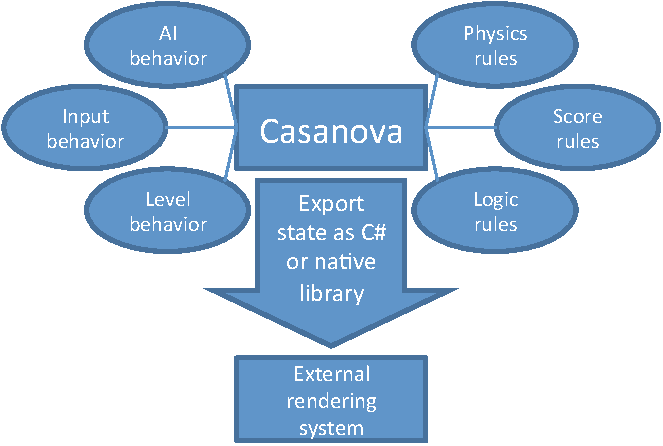
\includegraphics[width=0.5\textwidth]{architecture.pdf}
\caption{Game architecture with Casanova}
\noindent
%\hrulefill
\label{test}
\end{wrapfigure}

Behaviors are used to make it easier to build complex input, articulated level logics or customized AI algorithms into the game. While Casanova does not (yet) integrate any deduction engine or proper AI system, it makes integrating such a system with the game loop and the game state much simpler.

Rules are used to build all the regular logic that the game continuously repeats, for example the fact that when projectiles collide with an asteroid then the asteroid is damaged or other logical relationships between entities. Rules are the main workhorse of a game, and Casanova ensures that all the queries that make up the various rules maintain the integrity of the state and are automatically optimized to yield faster runtime.

The Casanova compiler will then export the game state as a series of type definitions and classes that can be accessed directly (that is without any overhead) from a C\# or C++ rendering library; this way existing rendering code and engines can be integrated with Casanova with little effort.
 

\section{The Casanova language}
\label{sec:casanova}
%%%%%%%%%%%%%%%%%%%%%%%%%%%%%%%%%%%%%%%%
% THE CASANOVA LANGUAGE
%%%%%%%%%%%%%%%%%%%%%%%%%%%%%%%%%%%%%%%%

In this section we present the Casanova language; for a more detailed treatment, see \cite{CASANOVA_TR}. Casanova is inspired to the ML family of languages.

\subsection{Design Goals}
We have designed the Casanova language with multiple goals in mind. First of all, Casanova games must be easy and intuitive to describe. For this reason we have used a mix of declarative and procedural programming. For expressing rules, declarative programming is simple, allows the developer to focus on what he wants to achieve rather than how, and there is a wealth of powerful optimization techniques for declarative operations on sequences of values coming from the field of databases \cite{QUERY_OPT}. The declarative portions of a game are all executed in parallel, and can take advantage of multi-core CPUs.

Procedural programming, in particular coroutines \cite{COROUTINES}, are used to describe computations that take place during many ticks of the game engine. Imperative coroutines are used to express the behaviors of a game. These behaviors are executed sequentially and with no optimizations, since they can access any portion of the state both for reading and writing, and they may perform any kind of operation.


\subsection{A brief introduction to Casanova}
Casanova is a programming language designed aroung a set of core principles aimed at aiding game development. Here we describe the language ``at a glance'', by listing its features designed to simplify repetitive, complex or error prone game coding activities: \textit{(i)} Casanova integrates the game loop and time as first-class constructs. The game loop and time management are almost always an important part of game development libraries, for example see \cite{XNA}; \textit{(ii)} it performs a series of optimizations that are usually found hand-coded in virtually all game engines \cite{GAME_OPT}, such as logical optimization of queries on lists and spatial partitioning/use of indices to speed up quadratic queries such as collision detection (for example: \texttt{colliders(self) = [other | other <- Others, collides(self,other)]}; \textit{(iii)} it guarantees that updates to the game state during one tick are consistent, that is the state is never partially updated thanks to a (high-performance) transactional system; \textit{(iv)} it offers a scripting system that integrates seamlessly with the update loop.

We have designed Casanova with the aim of adding more features such as: \textit{(i)} automated generation of all the rendering code; \textit{(ii)} automated generation of all the networking code; \textit{(iii)} automated generation of all or parts of an AI system.

Of course the language can also serve as a general purpose language. Any application that requires performing computations and visualization on a complex set of data which evolves over time according to a set of fixed rules might benefit from using Casanova. In the future we may investigate other possible uses of the language in this direction.
As a final remark,it must be noted that Casanova sometimes constrains the developer; for example, at most one rule may be associated with any given field of the game state and rules are always applied at every tick of the simulation. Since developers may find this set of restrictions too tight we have included a scripting system which can also act as a ``wildcard'' in this  regard, that is scripts have essentially no limitations in expressivity (scripts are a general purpose programming language with coroutines) and for this reason they can be used to express anything that the rule system cannot, albeit renouncing various useful features such as automated optimization.

\subsection{Syntax, Semantics and Types}
The details of the Casanova language syntax, semantics and type system are defined in \cite{CASANOVA_TR}. In this subsection we give a general overview of the most salient aspects of the language.

A Casanova program is divided into three parts: \textit{(i)} the state definition, \textit{(ii)} the initial state and \textit{(iii)} the main behavior.

The state definition contains the type definitions of the game state and game entities, together with the rules the various fields are subjected to. Rules may be nested, that is a field may contain a rule of type \texttt{Rule T}, where \texttt{T} contains a value of type \texttt{Rule V}. This is quite common, and we will seen an instance of this in the example below (in the \texttt{Introductory Example} subsection).

Entities and the state may be defined in terms of the usual type constructors found in a functional language: records, tuples and discriminated unions. Also, we can define values of type: table (for sequences), variable (for mutable cells), rule (for updateable fields) and reference (for read-only pointers).

The initial state defines the starting value of the various game entities.

The main behavior is an imperative process which runs for the entire duration of the game. A behavior may spawn (\texttt{run}) other behaviors, suspend itself for one or more ticks (\texttt{yield} or \texttt{wait}) or wait for another behavior to complete before resuming its execution (\texttt{do!} or \texttt{let!}). In addition behaviors may access the state without any limitation; a behavior can read or write any portion of the state: \texttt{:=} is the assignment operator and \texttt{!} is the lookup operator.

Behaviors can be combined with a small set of operators that define a simple concurrent calculus: \texttt{parallel x y}, which runs two behaviors in parallel and returns the pair with their results; \texttt{concurrent x y}, which runs two behaviors in parallel and returns the result of the first to terminate; \texttt{x => y}, which runs behavior \texttt{y v} only when \texttt{x} terminates with result \texttt{Some v}; and \texttt{repeat x}, which continuosly runs a behavior.

The tick function of the game is built automatically by the Casanova compiler, and it executes all running behaviors until they \texttt{yield}; then it executes all rules (in parallel and without modifying the current game state to avoid interferences); finally it creates the new state from the result of the rules.

Rules do not interfere with each other, since they may not execute imperative code. If rules immediately modified the current state, then their correctness would depend on a specific order of execution. Specifying said order would place an additional burden on the programmer's shoulders.

The tick function for rules presents a problem which is partly addressed with \texttt{references}: portions of the state must not be duplicated, for correctness reasons. This means that each entity in Casanova may be subjected to some rules but only once; if an entity is referenced more than once then it may be subjected to more (and possibly even contradictory) rules. For this reason we make any value of type \texttt{Rule} (or which contains a field of type \texttt{Rule}) linear \cite{LIN_TYPES}. This means that a value of type \texttt{Rule T} may be used at most once, and after it is read or used it goes out of scope.

We use the type constructor \texttt{Ref T} to denote a reference to a value of type \texttt{T}. A reference is a shallow copy to an entity which primary value is stored elsewhere. This allows for the explicit sharing of portions of the game state without duplication of rules, since rules are not applied to references. This also allows for safe cyclical references, such as:

\begin{lstlisting} 
type Asteroid = { ... Colliders : Rule(Table(Ref Projectile)) }
type Projectile = { ... Colliders : Rule(Table(Ref Asteroid)) }
\end{lstlisting} 

This restriction is enforced statically during type checking, and it ensures that all rules are executed exactly once for each entity.

The type checker enforces another property: a behavior gives a compile-time error unless it is statically known that all code paths yield. This is achieved by requiring that \texttt{repeat} and \texttt{=>} are never invoked on a behavior which does not yield in all its paths. For example, behaviors such as:

\begin{lstlisting} 
repeat { if !x > 0 then yield else y := 10 }
\end{lstlisting} 

generate a compile-time error.

This ensures that the tick function will always terminate, because rules are non-recursive functions and behaviors are required to never run without yielding indefinitely.


%%%%%%%%%%%%%%%%%%%%%%%%%%%%%%%%
%edit
%%%%%%%%%%%%%%%%%%%%%%%%%%%%%%%%
Of course it is possible to lift this restriction, since it may give some false negatives; for this reason, the actual Casanova compiler will be configurable to give just a warning instead of an error when it appears that a script does not yield correctly, to leave more freedom to those developers who need it.


So far the Casanova language enforces the following properties:
\begin{itemize}
\item developers do not have to write the boilerplate code of traversing the state and updating its portions; this happens thanks to the fact that Casanova automatically builds the game loop
\item all entities of the state are updated exactly once (even though they may be shared freely across the state as \texttt{Ref}s); this happens thanks to the linearity of the \texttt{Rule} datatype and the automatic execution of all rules by the game loop
\item rules do not interfere and are processed simultaneously; this happens thanks to the linearity of the \texttt{Rule} datatype and thanks to the fact that the state is created anew at each tick
\item the tick function always terminates; this happens because the state is not recursive (again, thanks to the linearity of \texttt{Rule}) and because our coroutines are statically required to always invoke \texttt{yield}
\end{itemize}

These properties alone are the correctness properties and ensure that the game will behave correctly. We will now see an example Casanova game. We will also see the set of optimizations implemented by the Casanova compiler, that make sure that a game runs fast with no effort on the part of the developer.


\subsection{Introductory Example}
A Casanova program starts with the definition of the game state, the various entities and their rules. A field of an entity may have type \texttt{Rule T} for some type \texttt{T}. This means that such field will contain a value of type \texttt{T}, and will be associated with a function of type: $ \mathtt{Ref(GameState)} \times \mathtt{Ref(Entity)} \times \mathtt{T}  \times \Delta \mathtt{Time} \rightarrow \mathtt{T} $

This function is the \textit{rule function}, and its parameters are (they can be omitted by writing an underscore \texttt{\_} in their position) \textit{(i)} the current state of the game; \textit{(ii)} the current value of the entity we are processing; \textit{(iii)} the current value of the field we are processing; \textit{(iv)} the number of seconds since the last tick.

When a field does not have an explicit rule function, then the identity rule is assumed. A rule function returns the new value of a field, and cannot write any portion of the state. Indeed, the current value of the state and the current entity are readonly inside the body of a rule function to avoid read-write dependencies between rules.

Updating the state means that all its rule functions are executed, and their results stored in separate locations. When all rule functions are executed, then the new state is assembled from their results.

In the remainder of the paper we will omit some type annotations; this is possible because we assume the presence of type inference.

In a field declaration, the \texttt{:} operator means ``has type'', while the \texttt{::} operator specifies the rule function associated with a rule.

The \texttt{!} operator is the dereferencing operator for rules, and it has type \texttt{Rule T -> T}.

Let us show how we would build a very simple game where asteroids fall down from the screen and are removed when they reach the bottom of the screen:

\begin{lstlisting}
type Asteroid = {
    Y     : Rule float :: fun (_,self,y,dt) -> y + dt * self.VelY
    VelY  : float        
    X     : float }

type GameState = {
    Asteroids           
        : Rule(Table Asteroid)
        :: fun (_,_,asteroids,_) -> [a | a <- asteroids && a.Y > 0]  	    
    DestroyedAsteroids	
        : Rule int
        :: fun (_,self,destroyed_asteroids,_) -> destroyed_asteroids + count([a | a <- !self.Asteroids && a.Y <= 0]) }
\end{lstlisting}
  
In the state definition above we can see that the state is comprised by a set of asteroids which are removed when they reach the bottom. Removing these asteroids increments a counter, which is essentially the ``score'' of our pseudo-game. Each asteroid moves according to its velocity.

The initial state is then provided:
\begin{lstlisting}
let state0 = { Asteroids = []; DestroyedAsteroids = 0 }
\end{lstlisting}

Behaviors in Casanova are based on coroutines, that is they are imperative procedures which may invoke the \texttt{yield} operator. Yielding inside a behavior suspends it until the next tick of the game. Behaviors may freely access the state for writing, that is behaviors are less constrained than rules but for this reason they also support less optimizations. The only requirement that Casanova enforces in behaviors is that they must never iterate indefinitely without yielding, and this requirement is verified with a dataflow analysis.

When the main behavior of a game terminates, the game quits.

The main behavior of our game spawns asteroids every 1-3 seconds until the number of destroyed asteroids reaches 100. The main behavior of our game is defined as:

\begin{lstlisting}
let main state =
  let rec behavior() = {
      do! wait (random.Next(1,3))
      state.Asteroids.Add { X = random(-1,+1); Y = 1; VelY  = random(-0.1,-0.2) }
      if !state.DestroyedAsteroids < 100 then do! behavior() else return () }
  in behavior()
\end{lstlisting}
  
The imperative syntax loosely follows the monadic \cite{MOGGI_MON,COMPR_MON} syntax of the F\# language, where a monadic block is declared within \texttt{\{\}} parentheses, and combining behaviors is done with either \texttt{do!} or \texttt{let!} and returning a result is done with the \texttt{return} statement. This allows us to clearly mark the points where a behavior waits for another behavior to complete before taking its result and proceding.


\subsection{Optimization}

Casanova is designed to make it easy to automatically perform three main optimizations: memory recycling, rule parallelization and query optimization.

Memory recycling, is a simple yet effective optimization for all those platforms (such as the Xbox 360) with a slow garbage collector \cite{XBOX_GC}. Memory recycling means that \texttt{Rule T} fields allocate a double buffer for storing both the current and the next value for rules, instead of regenerating a new state at each tick.
Rule parallelization is made possible by the static constraint that rules are linear: this means that no rules write the same memory location. We also know that rules may not freely write any references. These two facts guarantee thread safety, that is we may run all rules in parallel. 
The final optimization is query optimization. Nested list comprehensions (also known as ``joins'' in the field of databases \cite{QUERY_OPT}) can have high computational costs, such as $O(n^2)$, for example when finding all the projectiles that collide with asteroids. Such a complexity is unacceptable when we start having a large number of asteroids and projectiles, because it may severely limit the maximum number of entities supported by the game.
We use the same physical optimization techniques used in modern databases: we build a spatial partitioning index (such as a quad-, oc-, R-, etc. tree) to speed up our collision detection. The resulting complexity of the same query with a spatial partitioning index is $O(n \log n)$, which executes much faster and allows us to support larger numbers of entities.


\subsection{A Full Example}

We now show a full example of a game where a series of balls are thrown from one side of the screen and bounce towards the other side; the balls are removed when they reach the other side of the screen.

We start by defining the state (a collection of balls) and its rules (gravity, motion and removal of those balls that reach one side of the screen):
\begin{lstlisting}
let g = Vector2(-9.81,0.0)

type BallsState = {
    Balls     : Rule(Table Ball))
              :: fun (_,_,balls,_) -> [b | b <- balls && b.X <= 50.0 ] }
type Ball = {
    Position  : Rule Vector2
              :: fun (_,ball,p,dt) ->
                     if p.Y < 0.0 then Vector2(p.X, 0.0) 
                     else p + !ball.Velocity * dt

    Velocity  : Rule Vector2
              :: fun (_,ball,v,dt) ->
                     if p.Y < 0.0 then Vector2(v.X, -v.Y) * 0.6 
                     else v + g * dt }
\end{lstlisting}

Then we define the initial state, which does not contain any balls:
\begin{lstlisting}
let state0 = { Balls = [] }
\end{lstlisting}

Finally we define the main behavior which launches the balls, one every second:
\begin{lstlisting}
let rec main state = {
    do! wait 1.0
    state.Balls.Add { Position = Vector2(0.0, 0.0); Velocity = Vector2(5.0, 10.0) }
    do! main state }
\end{lstlisting}


\section{Case Study}
\label{sec:case_study}
Mini Galaxy Wars.

\section{Conclusions}
\label{sec:conclusions}
%%%%%%%%%%%%%%%%%%%%%%%%%%%%%%%%%%%%%%%%%%%%%%%%%%%%%%%%%%
% conclusions.tex
%%%%%%%%%%%%%%%%%%%%%%%%%%%%%%%%%%%%%%%%%%%%%%%%%%%%%%%%%%

Scripts are an important and pervasive aspect of computer games. Scripts simplify the interaction with computer game engines to the point that a designer or an end-user can easily customize gameplay. Scripting languages must support coroutines because these are a very recurring pattern when creating gameplay modules. Scripts should be fast at runtime because games need to run at interactive framerates. Finally, the scripting runtime should be as modular and as programmable as possible to facilitate its integration in an existing game engine.

In this paper we have shown how to use meta-programming facilities (in particular monads) in the functional language F\# to enhance the existing scripting systems which are based on Lua, the current state of the art, in terms of speed, safety and extensibility. We have also shown how having a typed representation of coroutines promotes building powerful libraries of combinators that abstract many common patterns found in scripts. As evidence of the capabilities of our proposed system we have outlined a series of applications of our scripts into an actual game that is under development.
 

\bibliographystyle{plain}
\bibliography{references} 

%\cite{*}
\nocite{}

\end{document}
